\documentclass[12pt, a4paper, unicode]{report}
% \usepackage[english]{babel}
\usepackage[utf8]{inputenc}

\usepackage{amsmath}
\usepackage{enumitem}
\usepackage{wrapfig}
\usepackage{tabto}
\usepackage{subcaption}
\usepackage{mathtools}
\usepackage{color}
\usepackage{authblk}
\usepackage{booktabs}
\usepackage{multirow}
\usepackage{setspace}





%%\usepackage{mathptmx} %% TimesNewRoman font style
\usepackage{ifthen}     %% If then else
\usepackage{verbatim}   %% For printing latex code
\usepackage{etoolbox}   %% Bibliography chapter to section
\usepackage{epigraph}   %% Adding text to part pages
\usepackage{graphicx}   %% Sample images
\usepackage{longtable}  %% Tables spanning more pages
\usepackage{ragged2e}   %% Alignment of quotes
\usepackage{datetime}   %% Date
\usepackage{graphicx}
\usepackage{listings}
\usepackage{dirtytalk}
\usepackage{float}
\graphicspath{./figures/images/}
% \restylefloat{table}
\usepackage[table,xcdraw]{xcolor}
\usepackage[hypertexnames=false]{hyperref}
\usepackage[all]{hypcap}%% Hyperlinks to the beginning of the figure
\usepackage{titlesec}  %% Customize chapters and sections
\bibliographystyle{ieeetr}
\usepackage[ruled,vlined]{algorithm2e}
%\usepackage[]{biblatex}
%\setlength\bibitemsep{1.5\baselineskip}

%\addbibresource{ms.bib}


\usepackage{xcolor}

\definecolor{codegreen}{rgb}{0,0.6,0}
\definecolor{codegray}{rgb}{0.5,0.5,0.5}
\definecolor{codepurple}{rgb}{0.58,0,0.82}
\definecolor{backcolour}{rgb}{0.95,0.95,0.92}

\lstdefinestyle{mystyle}{
	backgroundcolor=\color{backcolour},   
	commentstyle=\color{codegreen},
	keywordstyle=\color{magenta},
	numberstyle=\tiny\color{codegray},
	stringstyle=\color{codepurple},
	basicstyle=\ttfamily\footnotesize,
	breakatwhitespace=false,         
	breaklines=true,                 
	captionpos=b,                    
	keepspaces=true,                 
	numbers=left,                    
	numbersep=5pt,                  
	showspaces=false,                
	showstringspaces=false,
	showtabs=false,                  
	tabsize=2
}

\lstset{style=mystyle}

\usepackage{geometry}
 \geometry{
 top=25mm,
 bottom=25mm,
 left=37mm,
 right=25mm
 }
 
%%%%%%%% List of Acronyms %%%%%%%%

\usepackage[acronym, toc]{glossaries}
\makeglossaries

\newacronym{seda}{SEDA}{Staged Event Deriven Architecture}
\newacronym{SYMPED}{SYMPED}{SYmmetric Multi-Processor Event Driven}
\newacronym{NIO}{NIO}{Non Blocking IO}
\newacronym{OIO}{OIO}{Old IO}
\newacronym{VM}{VM}{Virtual Machine}
\newacronym{gcloud}{gcloud}{Google Cloud}
\newacronym{AST}{AST}{Abstract Syntax Tree}
\newacronym{MAPE}{MAPE}{Mean Absolute Percentage Error}
\newacronym{MSE}{MSE}{Mean Squred Error}



%%%%%%%%%%%%%%%%%%%%%%%%%%%%%%%%%%%

\renewcommand{\baselinestretch}{1.5}

% Document information
\author{By\\ L A S J Gunasekara \\Supervised by\\Dr. Chamath Keppitiyagama}

\date{\monthname\ \the\year}

\begin{document}

\begin{titlepage}
\newgeometry{top=3.15in,bottom=1.97in,right=1.25in,left=1.25in}
   \begin{center}

        \textbf{\Huge Machine learning approach to fine-tune Ballerina thread pool size}
        \vfill
        \LARGE{Lakindu Akash}

   \end{center}
\end{titlepage}
\begin{titlepage}
	\newgeometry{top=1in,bottom=1in,right=1in,left=1in}
	\begin{center}
		
		
\includegraphics[width=0.15\textwidth]{figures/UoC-logo-black.png}
		
		\vspace{1.5cm}
		
		\textbf{\huge Machine learning approach to fine-tune Ballerina thread pool size}
		
		\vspace{3cm}
		\textbf{\Large{L A S J Gunasekara}}\\
		\textbf{\Large{Index No : 16000536}}
		
		\vspace{3cm}
		\textbf{\Large{Supervisor: Dr. Chamath Keppitiyagama}}\\
		\textbf{\Large{Co-Supervisor: Dr. Malith Jaysinghe}}
		
		
		\vspace{1.5cm}
		
\includegraphics[width=0.15\textwidth]{figures/UCSC_Logo.jpg}
		\vspace{1cm}\\
		\textbf{\Large{January 2021}}
		
		\large{Submitted in partial fulfillment of the requirements of the\\
			B.Sc in Computer Science Final Year Project (SCS4124)}
		
		
		\vspace{0.7cm}
		
		
		
	\end{center}
\end{titlepage}

\pagenumbering{roman}

\chapter*{Declaration}

I certify that this dissertation does not incorporate, without acknowledgement, any material previously submitted for a degree or diploma in any university and to the best of my knowledge and belief, it does not contain any material previously published or written by another person or myself except where due reference is made in the text. I also hereby give consent for my dissertation, if accepted, be made available for photocopying and for interlibrary loans, and for the title and abstract to be made available to outside organizations.
\\\\
Candidate Name: L A S J Gunasekara
\\\\\\
....................................\\
Signature of Candidate
\hspace*{.5\textwidth} Date: 07/02/2021
\\\\
This is to certify that this dissertation is based on the work of 
Mr. L A S J Gunasekara under my supervision. The thesis has been prepared according to the format stipulated and is of acceptable standard.
\\\\
Principle Supervisor’s Name: Dr. Chamath Keppitiyagama \\ 
Co- Supervisor’s Name: \hspace*{.055\textwidth} Dr.  Malith Jayasinghe
\\\\\\
....................................\\
Signature of Supervisor
\hspace*{.5\textwidth} Date: 07/02/2021
\chapter*{Abstract}

Modern web servers use various techniques to achieve high performance. Every web server applications use a thread pool to distribute the workload. Performance of such servers are highly dependent on the number of threads in the worker thread pool. The optimal thread pool size is dependent on multiple factors. Type of workload (nature of
user application/ implementation) is one key factor of that. This paper propose a technique to identify optimal thread pool size for the user program based on the program features using a machine learning approach.

\chapter*{Preface}

The purpose of this dissertation is to present the work from the research named "Machine learning approach to fine-tune Ballerina thread pool size". Final solution includes a machine learning model that estimate the thread pool size of Ballerina scheduler based on program features. Starting point of this study was comparing performance between different server architectures in Ballerina and evaluating performance for different types of Ballerina programs. Then discussed how to improve performance further for different programs especially for programs that consists of different types of IO features. It is identified thread pool optimization is the best way to improve the performance. Experiments were run in each phase and results were justified. Finally, it is shown that predicted thread pool size from the machine learning model is better than the current Ballerina architecture. There were no performance comparison done for different sever architectures and for different thread pool size for Ballerina language. Furthermore, no study were conduct to extract features from the source code and estimate the parameters that would give the best performance for a web server. 

My original works include implementing different server architectures for ballerina, performance comparison of each other, identification of different prgram features that affect the performance of web server, implementation of many different programs in order to train the machine learning model, and implementing a machine learning model that predict the optimal thread pool size.
\chapter*{Acknowledgment}

I would like to extend my sincere gratitude to my supervisor Dr. Chamath Keppetiyagama and my co-supervisor Dr. Malith Jayasinghe for guiding me throughout the research.

\newpage
\tableofcontents

\newpage
\listoffigures
\listoftables
\printglossary[title=List of Acronyms, type=\acronymtype]

%%%%%%%%%%%%%%%%%%%%%%%%%%%%%%%%%%%%%%%%%%%%%%%%%%%%%%%%%%%%%%%%%
% CHAPTERS
%%%%%%%%%%%%%%%%%%%%%%%%%%%%%%%%%%%%%%%%%%%%%%%%%%%%%%%%%%%%%%%%%

\newpage
\pagenumbering{arabic}

\chapter{Introduction}

This research was able to explore various optimization techniques based on programming features. Initially this research started with idea of finding optimal web server architecture based on programming features of Ballerina language. With extensive tuning of Ballerina's internal architecture it was able to identify tuning the thread pool size of the existing architecture is the best way maximize the performance for given program.

\section{Background to the Research}

Web server optimization is prominent branch in the enterprise level software industry. Optimization aids to utilize the resources efficiently for web servers. This research came along long way and narrowed down from web server architecture implementation to thread pool optimization using programming features in Ballerina language. Prior determination of web sever architecture that perform best is difficult due to various factors such as type of workload that process, working environment \cite{comp_ac} etc. It is challenging to provide the best architecture for all type of workload \cite{seda,events_are_bad,edprs} because implementation of framework and language affect the performance as well.Also, there is no knowing mechanism to identify the type of workload prior to the execution of program and selecting best web server architecture for identified workload. 

\newpage

\section{Research Problem and Research Questions}

This research addresses the following questions.


\begin{itemize}
 \item Is it possible to tune Ballerina's internal server architecture to maximize the performance for given type of workload?
 \item Is it possible to propose optimal web server architecture based on program features?
\end{itemize}


%%\begin{figure}[htbp]
%%  \begin{center}
%%    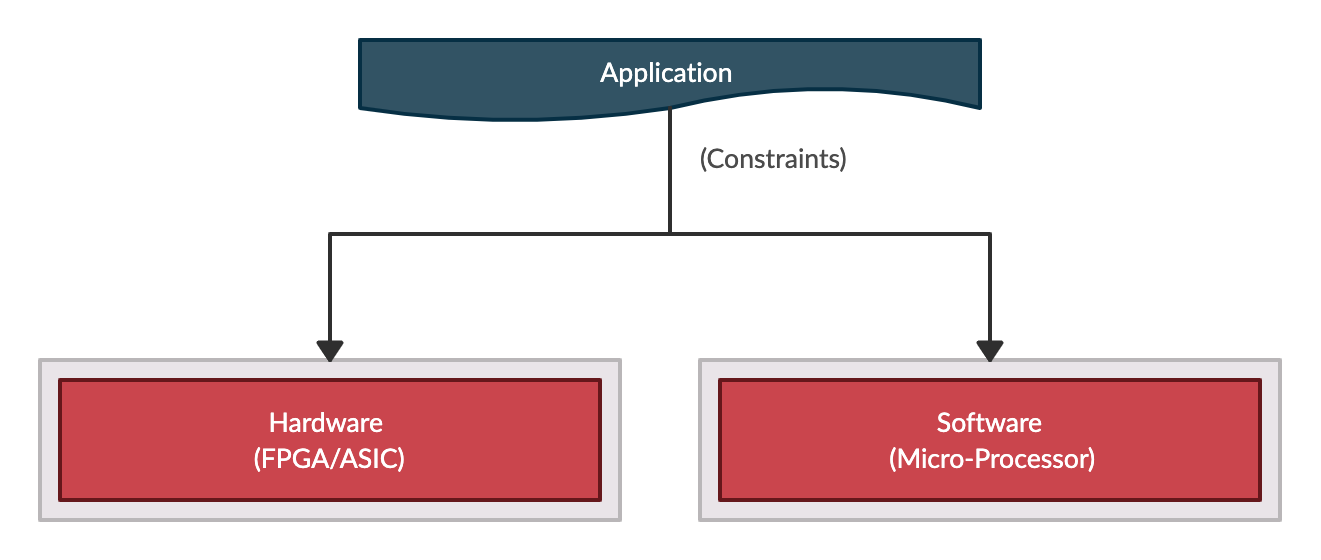
\includegraphics[scale=0.3]{images/problem.png}
%%    \end{center}
%%  \caption{HW/SW Paritioning problem}
%%\end{figure}


\section{Justification for the research}

 In the previous researches, they tried to provide optimal web server architecture for offered workload. Also, there is no global model to generalize the findings of those researches. This research tries to find model to predict optimal web server architecture for given program for the Ballerina language which is designed for network programming.  Also, there are a number of researches for thread pool tuning with black box and white box approaches. All approaches have their own advantages and disadvantages. This research proposes technique using machine learning to find optimal thread pool size for given program.  
 
 None of previous researches have been automated the identification of programming features automatically and the propose the optimal thread pool size or web server architecture that given set of features or user program. Ballerina is better candidate for the research because identification of the programming features is more convenient because, features that are harder to extract in other languages are part of the Ballerina language.  


\section{Methodology}

	This research started with implementing new web sever architectures in Ballerina and then evaluating the performance of each including the existing architecture (Look figure \ref{bal_internal}). These architectures are inspired from Thread per connection model and event based models(Ex: \acrshort{seda}). This step includes modifying the Ballerina source code. Proper implementation requires deep analysis of Ballerina run time and optimization for the implementations, otherwise bugs can affect the performance. 
	
	Performance are evaluated with test programs which consist of different programming features. As an example one program may consists of several database calls and another program only contain the some arithmetic operations. Then performance are evaluated according to program features. The target is to provide best performant architecture for given features. Fine-tunes are carried out based on results of each phase. That led the research to focus on thread pool tuning after number of experiments. 
	
	Final model is consisted of a machine learning model that provide optimal thread pool size for given program. Figure  \ref{hl_architecture} shows the overview of the research. Results are dependent of the deployment environment of the service. Hence, first user need to train the machine learning model with predefined set of programs. The user able to provide own program and the model predict the optimal thread pool size for that program. These steps are explained more detail in Chapter 3.   
	
	\begin{figure}[htbp]
		\begin{center}
			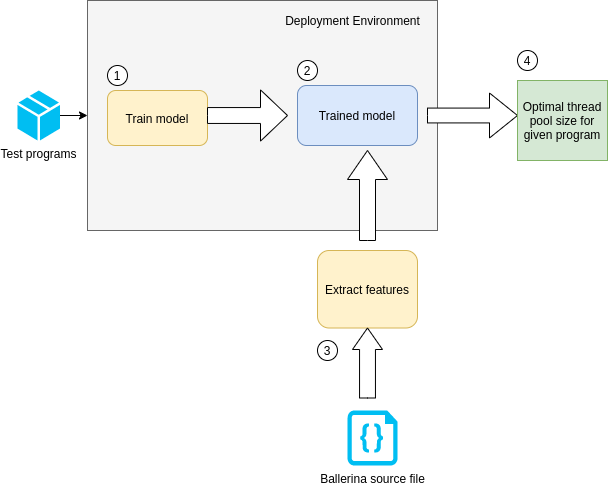
\includegraphics[scale=0.5]{figures/hl_architecture.png}
		\end{center}
		\caption{High-level overview of the research}
		\label{hl_architecture}
	\end{figure}
	

\section{Outline of the Dissertation}

This dissertation outlines 6 chapters as follows.

\begin{enumerate}
	\item Introduction
	\item Literature Review 
	\item Research Design
	\item Implementation
	\item Results \& Evaluation - Contain the results obtained in each phase and in depth discussion of the results.
	\item Conclusion - Discuss how the results mentioned in Chapter 5 has addressed the research questions. An emphasis will be given in highlighting the contribution of this research work to the scientific world. Implications of further research will also be discussed in this chapter.
\end{enumerate}

\section{Definitions}

\subsubsection{Concurrency level}

Concurrency level refer the concurrent number of users which are connected a web service.

\subsubsection{Deployment environment}

Deployment environment is where web server and all the experiments are running. Results are subjects to the configurations of that environment. Configuration of the environment includes the Operating system, Number of CPU core, Speed of the CPU, Amount of RAM and Network stability.

\section{Delimitations of Scope}

\subsection{In-Scope}

\begin{itemize}
	\item Introduce new architectures to existing Ballerina run time
	\item Fine tune and optimise the each architecture - Fine tuning includes the changing thread pool size.
	\item Take measures to keep accuracy of the experiments by monitoring the testing environment, isolating the resources etc.
\end{itemize}

\subsection{Out-Scope}

\begin{itemize}
	\item Generalizing the findings for other languages and frameworks
	\item Evaluate and compare the model in different environments.
\end{itemize}

\section{Conclusion}	

This chapter provides base principles and presents a foundation to the dissertation. At the beginning, the research problem was identified, formulated research questions, and research was justified. Then the definitions were presented, dissertation was outlined, research design and implementation was briefly discussed laying the path to proceed with detailed explanation of the research.
\chapter{Literature Review}\label{chap:2}

\section{Overview}

This section provides a broader context of this area concerning other researches and studies. The literature review consists of the following areas. 

\begin{enumerate}
	\item Characteristics of IO 
	\item Performance of web server architectures
	\item Importance of thread pool tuning
	\item Appropriateness of Ballerina for this research
	
\end{enumerate}

\begin{comment}
	Following few sections span some core topics related to the research and effort of other researches who put in this area.
	
	A web server needs to support millions of users demanding access to services that must be responsive,
	robust, and always available. The number of concurrent sessions and hits per day to web servers
	translates into an even higher number of I/O and network requests, placing enormous demands on
	underlying resources. 
	
	This research started with boarder area of web server architecture optimizations. The aim was to identify optimal web server architecture in Ballerina for given type of workload or program. Exploration mainly started with identifying IO features of the programs when classifying the workload. Then this research able to identify prominent IO features in Ballerina using extensive testing. Based on those IO features this research able to propose optimal thread pool size using machine learning algorithms. Finally narrowed down to finding the optimal number of threads in thread pool for given program.
\end{comment}




\section{Background and related theories}

\subsection{About IO}

Basically, every program instruction can be divided into IO and non-IO operations. IO operations are
typically operations that do not use the CPU. When there is an API call that requests data from IO,
that call won’t immediately return, but with some delay. \cite{nb_algo} This delay can be very small for
requesting a file on a hard drive, and much longer when requesting data from a network. This is
because the data that is requested from IO devices has to travel longer to the caller. For example, a call to an external HTTP server has to wait more rather than requesting data from a server where hosted on the same machine.
There are two types of IO,

\begin{enumerate}
	\item Blocking IO
	\item Non-blocking IO
\end{enumerate}

Calling an operation that requests data from IO will cause the running thread to "block", i.e. it is
waiting until the requested data has returned to the caller. When a thread is blocked in Linux, it will be put in a Sleep state by the kernel
until data has returned to the caller. Threads in sleep state immediately give up their access to the CPU,
so as to not waste CPU time. After IO is ready, the thread is taken out from the Sleep state and put in a
Runnable state. Threads in this state are eligible to be executed on the CPU again. The thread
scheduler will put the thread on a CPU when one is available. The process of taking threads on and off
the CPU is called context switching where this process is done at OS level. Context switching is quite expensive because it has to save the data related to its state called context and when it is ready to run, data must be restored again into CPU registers and stacks. The allocated memory size of thread in java is 1 Mb by default. A web server receiving 1000 concurrent requests may result in 1000Mb usage of RAM only to maintain the thread. Moreover, when there is a large number of context switching is happening larger overhead is added to the system. This is where the disadvantage of the thread per connection model is apparent.

Non-blocking IO reduces the context switching by reusing the threads. The main benefit of non-blocking IO
is that we need fewer threads to handle the same amount of IO requests. When there is an IO operation that needs to be performed, the task is delegated to OS and so that call is kept in a queue, then thread is released for other operations. When IO is completed, the queue is notified and further instructions of the task are carried out afterward. Non-blocking IO is tightly coupled with thread pools. The fewer threads are allocated in advance and tasks are executed by those threads by reusing. Therefore, context switching is minimized.

\subsection{Event loops}
To facilitate the non-blocking IO most programming languages implement an event loop. The concept
of the event can be any operation including IO operations needed to be executed. The event loop polls
(constantly check) if data is returned from IO. An event loop is a while(true) loop that in
each iteration will check if data is ready to read from a File Descriptor in Unix systems \cite{device_file}. The
list of File descriptors that we want to check for ready data is called the interest list. At glance, we can
think of the event loop as an expensive task. Although several optimization techniques have been implemented at the kernel level to reduce the cost of the event loop. Some examples are epoll,
io{\_}uring, kqueue \cite{web_pipeline,io_uring}.


\subsection{Web Server architecture performance}

There are several web server architectures which have existed for a long time. In the early 90s, the thread per connection model was popular because it is relatively easier to implement. But when the internet is getting popular, web servers get more hits. The thread per connection model has serious flaws when there are higher numbers of concurrency reaches. Since each thread needs a considerable amount of memory and overhead of context switching \cite{seda}. Having thousands of connections to such a server cannot handle large requests. In order to overcome this problem SEDA (Staged event driven architecture) \cite{seda} were proposed. It limits the thread count using the concept of using thread pools, thus it reduces the context switching and memory usage. SEDA is a very successful mechanism to handle large concurrencies. Although the question had arisen “do SEDA perform well in every situation?”. \cite{Scalable_Threads_for_Internet_Services,events_are_bad,event_deriven_programming_for_robust_software} This debate has a long history. To answer this there were several studies conducted and proposed several fine-tuned architectures for refined situations.

\textit{Bharti et al.} \cite{fine_grained_SEDA} proposed a fine Grained SEDA Architecture for Service-Oriented Network Management Systems in order to improve the performance architecture for specific functions. They are fine-tuning \acrshort{seda} by breaking the stage in SEDA into sub-stages. Each sub-stage represents a SEDA implementation of critical functionality of the parent SEDA stage where each stage consists of a single thread pool. In those stages, performance has been improved by micro-managing the functionalities of each sub stage. Hence, the application, instead of having a single stage with competing threads from their functionalities, will now have fine-grained sub-stages. Each of the fine-grained sub-stages will now host threads performing a much smaller set of tasks. They showed that design has significant performance improvement of the application. 

\textit{Pariag et al.} \cite{comp_ac}  showed extensive tuning of web server architectures able to significantly improve the performance of specific types of workloads. Workload refers to what type of operation expects to be carried out in the web server, especially IO operations. They have considered 3 different server libraries that have different server architectures, the $\mu$server utilizes an event-driven architecture, Knot that uses the highly-efficient Capriccio thread library for implementing a thread per connection model, and WatPipe that uses a hybrid of events and threads to implement a pipeline based server that is similar to staged event-driven architecture \acrfull{seda} server like Haboob \cite{seda}. They have modified the Capriccio thread library to use Linux's zero-copy sendfile interface. Then they have introduced the \acrfull{SYMPED} architecture in which relatively minor modifications are made to a single process event-driven (SPED) \cite{flash_server} server (the $\mu$server) to allow it to continue processing requests in the presence of blocking IO due to disk accesses. They finally describe a C++ implementation of WatPipe, which although utilizing a pipeline-based architecture, excludes the dynamic controls over event queues and thread pools used in SEDA. 

They have compared all three architectures and the conclusion is slightly different from the previous studies. One important conclusion of them related to this research is they have observed that when using blocking sockets to send data to clients, the performance obtained with some architectures is quite good and in one case is noticeably better than when using non-blocking sockets. They have shown that a proper combination of the number of connections and kernel-level worker threads (or processes) is required to get the best performance results for each workload type.

In their conclusion they have stated  “this work could be done after or in conjunction with work that enables servers to automatically and dynamically tune them-selves to efficiently execute the offered workload”

More recent similar works \cite{comparing_high_performance_multi_core,uniproc_multiproc} can be found regarding improving the performance of web server architectures. Thus, we can conclude the performance of web server architecture is dependent on the type of workload or type of operations which web server executes. Tuning parameters such as thread pool size of web server also able to improve the performance.

Behren et al. \cite{events_are_bad} claiming that “Events Are A Bad Idea (for high-concurrency servers)”. They have shown a comparison of benchmark results of threaded and event-based architectures. In their conclusion stated, “Although event systems have been used to obtain good performance in high concurrency systems, we have shown that similar or even higher performance can be achieved with threads”. But there is a question left on whether it holds true only for the Java \acrshort{NIO} library or for the non-blocking approach in general.

\subsection{Ballerina language}

As the growing needs of the distributed computing and rapid development of web services, new programming
languages and paradigms were emerged. Ballerina \cite{ballerina} is such a successful language that handles
network programming in a developer-friendly way. Here I quoted a small paragraph from the ballerina
website.

“For decades, programming languages have treated networks simply as I/O sources. Ballerina
introduces fundamental, new abstractions of client objects, services, resource functions, and listeners
to bring networking into the language so that programmers can directly address the Fallacies \cite{fallacies_of_distributed_computing} of
Distributed Computing as part of their application logic. This facilitates resilient, secure, performant
network applications to be within every programmer’s reach.”

Apart from the above quotation, Ballerina is best suited for this research since Ballerina language has certain capabilities extracting performance-critical features especially IO calls. In Ballerina, they are called connector calls. In order to answer the second research question, this provides huge benefits as network calls are first-class citizens in Ballerina languages. Chapter \ref{chap:3} explains more about these features.

While other languages provide network operations as library functions Ballerina provides in a native way. If we try to extract such features from other languages we need to know exactly which function call does an IO operation including library functions. That is a very difficult task to extract such features just by exploring the source code in other languages like C, Java, etc.

Network services are first-order objects in ballerina language similar functions. \cite{ballerina_book} Such features
can be used to identify whether a given program contains network services or not. In other languages, we need to have prior knowledge about which libraries are used for such implementations and which part of the code implements the network services.


There are some tools already developed \cite{ballerina_plugin_vs_code,ballerina_plugin_intelij} using these features in order to represent the code as sequence diagrams. Figure \ref{diagram_view_ballerina_code} shows a generated sequence diagram for a code that includes a remote database call.

 \begin{figure}[htbp]
	\begin{center}
		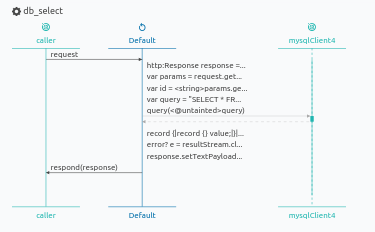
\includegraphics[scale=0.7]{figures/diagram_view_db_call.png}
	\end{center}
	\caption{Sequence diagram representation of code}
	\label{diagram_view_ballerina_code}
\end{figure}
 
It is clear that we can use the network awareness properties of the Ballerina language to identify
performance-critical features directly from source code, unlike other languages. Examples of network
awareness features are creating RESTful clients and servers, making database queries, completing
asynchronous calls, producing and consuming streaming data message-passing etc \cite{ballerina_book}.

\subsection{Thread pool tuning}

Thread pools are a very important component when implementing server architectures. In SEDA every stage has its own thread pool. Creating and destroying a thread is resource intensive task for the OS \cite{thread_pool_analysis}. Instead of creating and destroying threads on demand, thread pool reuses the allocated number of threads. The size of the thread pool is almost fixed, although there are many studies to propose the number of threads in the pool dynamically using various approaches in order to gain the performance. Some approaches propose analytical models and schemes \cite{xu2004performance,thread_pool_analysis,math_aproach_thread_pool_tuning,syer2011identifying,linfeng2017design} and other approaches use run-time information \cite{lorenzon2016investigating,nieplocha2007evaluating,agrawal2006adaptive} to predict size of the pool. Most server implementation decides the number of thread in the pool heuristically and based on empirical knowledge \cite{thread_pool_analysis,math_aproach_thread_pool_tuning} to get balanced performance for every type of operations including IO since integrating analytical modeling is complex and calculation of run-time information can add an overhead to the server.

When discussing some heuristic and experience based approaches to decide the thread pool size, one rule is that the size of the thread pool should be two times the number of CPUs (processors). Ballerina scheduler is also following this rule. Another rule, used by Microsoft's IIS, initially allocates 10 threads in the thread pool per CPU, and allows the size of the thread pool to increase based on the number of client requests \cite{thread_pool_analysis}. The thread pool's maximum size is heuristically set to be two times the number of megabytes of RAM in the host machine. Those heuristics are based on memory and CPU capabilities and there is no theoretical justification.

\textit{Yibei Ling} et al. \cite{thread_pool_analysis} propose a mathematical model to predict optimal thread pool size by calculating the cost of spawning, destroying and maintaining threads in a thread pool. However, this approach has some flaws because of the assumptions they initially made. The first assumption is that each thread in the pool has the same execution priority and receives uniform treatment. This is not always true because OS has a limited number of processors and there are other OS-level processes also using those resources. Typical modern web servers are deployed with resource control and monitoring tools as well. Thus threads may not get equal access to CPUs. The next assumption is one web request is very much like another and that the memory and I/O resources required by different threads are minimal. This research's major focus is to optimize the server architectures for different types of programming features especially IO. 

D.L. Freire et al.\cite{math_aproach_thread_pool_tuning} also did a similar study to calculate the expected gain of web servers under different thread pool sizes using an analytical model. The optimal size of the pool depends on the cost of creating threads, the cost of maintenance of the pool and the workload of the system as a probability density function. The workload can be thought of as the rate of receiving the client request to the web server. Experiments were evaluated under four different probability density functions which are uniform, exponential, density of Pareto and gamma density. Then optimal thread pool size is decided for each density function. However, this study has a similar assumption to the above study. 
 
There are a number of parameters that can be tuned in a thread pool such as number of threads in the pool, maximum number of threads allowed in a pool, maximum time interval that a thread will be idle waiting for a new task \cite{math_aproach_thread_pool_tuning}. However, most of the studies are focused only to tune the size of thread pool size since that parameter affects most when evaluating the performance of web servers.

\begin{comment}

\subsection{Static Program analysis for performance}

Program analysis can be divided into static analysis and dynamic analysis. There are some previous studies which have been put effort on static analysis and dynamic analysis for performance modeling while relatively fewer studies have been done for static analysis for performance modeling.  

\end{comment}

\subsection{Importance of optimization} 

Optimization for web server is important for a business, so services able to deliver better performance using minimum resources. Today, a larger portion of businesses are dependent on web services. Growing needs demand more resources that cost for the business. Although the word "optimization" shares the same root as "optimal", it is rare for the process of optimization to produce a truly optimal system. It is hard to define an optimal system where the system is optimized under certain quality metrics, which may be in contrast with other possible metrics. Therefore, the optimized system will typically only be optimal in one set of applications, not for all. One might reduce the CPU usage, while one is optimizing memory usage. Often there is no "one size fits all" design that works well in all cases, thus there are trade-offs to optimize the attributes of the greatest interest.

When coming into web server optimization, it can be achieved in different ways. One way is to write clever code that uses better data structures and algorithms, place code in perfect places in order not to waste CPU for IO. Programming patterns like asynchronous programming patterns provide some shortcuts for developers in order to overcome blocking scenarios. Still, optimization is hard for every aspect because interrelation of trade-off between techniques \cite{wescott2013every,Adewumi+2018+115+122}.  Another way is to optimize web servers where business logic is executing. Then developers able to focus more on business logic rather than spending time on code optimization.



\section{Conclusion}

It is clear that the performance of a web server can be depended on the type of operation that is carried out by the web server. Moreover, IO features affect the performance of web servers and some web server architectures perform well for certain use cases. Also, careful tuning of web servers was able to achieve significant performance improvement. Furthermore, thread pool tuning is dominant where the domain of optimizing the performance of server architectures. It is understandable why analytical models are sometimes not practical in certain situations. Finally, no research could be found that program classification is based on how programming features affect the performance of web servers.   

\begin{comment}

	Although the word "optimization" shares the same root as "optimal", it is rare for the process of optimization to produce a truly optimal system. A system can generally be made optimal not in absolute terms, but only with respect to a given quality metric, which may be in contrast with other possible metrics. As a result, the optimized system will typically only be optimal in one application or for one audience. One might reduce the amount of time that a program takes to perform some task at the price of making it consume more memory. In an application where memory space is at a premium, one might deliberately choose a slower algorithm in order to use less memory. Often there is no "one size fits all" design which works well in all cases, so engineers make trade-offs to optimize the attributes of greatest interest. Additionally, the effort required to make a piece of software completely optimal – incapable of any further improvement – is almost always more than is reasonable for the benefits that would be accrued; so the process of optimization may be halted before a completely optimal solution has been reached. Fortunately, it is often the case that the greatest improvements come early in the process.
	
	Even for a given quality metric (such as execution speed), most methods of optimization only improve the result; they have no pretense of producing optimal output. Superoptimization is the process of finding truly optimal output.
	
	\subsection{The IO and Programming}

	
	In early days one major reason to use blocking code (synchronous programming) is that it is easy to write
	programs. Programmer always knows the order of code which is executing. When there is a blocking IO call ,in most cases, the wait is not really a problem because the program can not perform anything else until the IO is finished. However, in cases such as network programming with multiple
	clients, the program may wish to perform other activity as it continues to wait for more concurrent
	users.
	One solution for these situations is to use multiple threads so that one part of the program is not
	waiting for unrelated IO to complete. But having many threads add large overhead to memory and
	CPU ( thread creation and context switching is costly)
	Another alternative is to use asynchronous programming techniques with non-blocking system calls.
	An asynchronous call returns immediately, without waiting for the IO to complete. The completion of
	the IO is later communicated to the application either through the setting of some variable in the application or through the triggering of a signal or call-back routine that is executed outside the linear
	control flow of the application.
	New programming languages and patterns have been adopted for exponential growth of web service
	requirements and rapid development. But utilizing the program to use it’s full potential and use
	resources efficiently is still a problem. Developers or programmers need to put more effort into
	optimizing the programs.
	One such optimization way is to write clever codes to use the blocking or waiting time on CPU for
	other tasks. In order to do that, programmers need to know where the IO calls happen. But using many
	libraries and knowing where the IO calls happen is a very complex task. Even though it could be
	found such calls optimizing is still hard.
	
\end{comment}







\chapter{Design}\label{chap:3}


This chapter undergoes the design steps that are taken in each stage of the research. Initially, this research is started as\textbf{ Compile time server architectures for Ballerina}. After analyzing the results of the initial set of experiments, the focus area is narrowed down to finding optimal thread pool size for different programming features. A machine learning approach is used to predict the thread pool size for a given set of programming features. Research questions remain unchanged from the beginning since thread pools are a crucial part of web server architectures and it is a tuning parameter for further improving the performance of server architecture. Literature review indicates that the performance of single web server architecture differs according to the type of operations it executes. Type of the operations can be extracted by analyzing the source code.  In simple terms, different web server architectures perform differently for different types of programs. Then based on the results further improvements and fine-tuning to the architecture are carried out in order to identify what parameters are required to change for maximizing the performance for each type of program. 

Formal research methodology is based on Design science research approach \cite{design_science}. Design science research approach requires the creation of an innovative, purposeful artifact for a special problem domain. The artifact must be evaluated in order to ensure its utility for the specified problem. In order to form a novel research contribution, the artifact must either solve a problem that has not yet been solved, or provide a more effective solution. Both the construction and evaluation of the artifact must be done rigorously, and the results of the research presented effectively both to technology-oriented and management-oriented audiences.


\begin{comment}
	This research tries to provide more effective solutions to a current problem and creates innovative solutions by introducing techniques to predict optimal thread pool size based on program features.
\end{comment}


The design of the research is divided into four stages. First off, existing Ballerina server architecture is carefully analyzed and designed how new architectures can be derived from it. New architectures are implemented by modifying the source code. Secondly, identified parameters from the first phase are tuned in order to maximize the performance in server architectures. In this phase, the size of the thread pool is tuned. Thirdly, differentiating the IO intensive features in the program and machine learning model is designed to predict the size of the thread pool. Afterward, \acrshort{AST} is parsed for extracting the identified features to feed into the machine learning model which is designed. 

This research consists of the following areas. The below sections span the design steps considered answering the research questions mentioned in the section.

Before diving into the design steps, it is important to specify the internal architecture of Ballerina run time. The next section briefly explains the internals of the Ballerina.



\section{Ballerina}\label{Sec_Ballerina}

This section provides an overview of current Ballerina architecture and explanation on how this research expects to use network awareness features in Ballerina language.  

In Ballerina connector calls that basically perform IO operations are explicitly presented in the source code as “ - $>$“. \acrfull{AST} parser extracts this information from the source to identify whether this call is a connector call and type of the connector call (HTTP, Database etc.).

Following is one example how the database calls are represented in ballerina code, note the -$>$ symbol.\\

\textit{stream$<$record{}, error$>$ resultStream = mysqlClient4 - $>$ query(<@untainted>query);}\\

Algorithm used for this operation is presented in section \ref{phase_iv}


\subsection{Ballerina internal architecture}

This section explains the main components of Ballerina run time.

\subsubsection{Netty Layer}

This layer is implemented using a library called Netty \cite{netty}. The primary task of the Netty layer is to listen for HTTP client connections and manage the session. It has its own thread pools to handle those connections. In original ballerina architecture, this layer simply handed over the incoming connection to the ballerina scheduler. Then the scheduler invokes relevant tasks for the client and returns the results to the Netty layer again for submitting back to the client. Inside the Netty layer, there are two types of threads. (1) \textbf{Boss threads} — Each bonded port has its own boss thread. For example, if the server listens on ports 80 and 443, then there are two boss threads. Main function of these threads is accepting the client requests. (2) \textbf{Worker threads} — Boss thread passes the accepted request to the worker thread. Worker threads then carries out the execution of the task. In Ballerina, these worker threads pass the request to the Ballerina scheduler.

\subsubsection{Scheduler}

Ballerina scheduler is the main component for every program/operation which executes. The Ballerina scheduler executes the client request using its own thread pool. The default thread pool size is two times the available processor count of the operating system. All the tasks which need to be executed are held in a queue. Then threads in the pool access the queue and execute the task. This is where major turnings are happening at the final stage of the research. 

\subsubsection{Resource function}

In Ballerina each API endpoint can be implemented as a resource function. That function includes all the implementation required to fulfill the task that the client is requested. More details about resource function are stated in chapter \ref{chap:4}. In this research, each resource function is considered a program.


Figure \ref{bal_internal} shows high level view of Ballerina architecture.

\begin{figure}[htbp]
	\begin{center}
		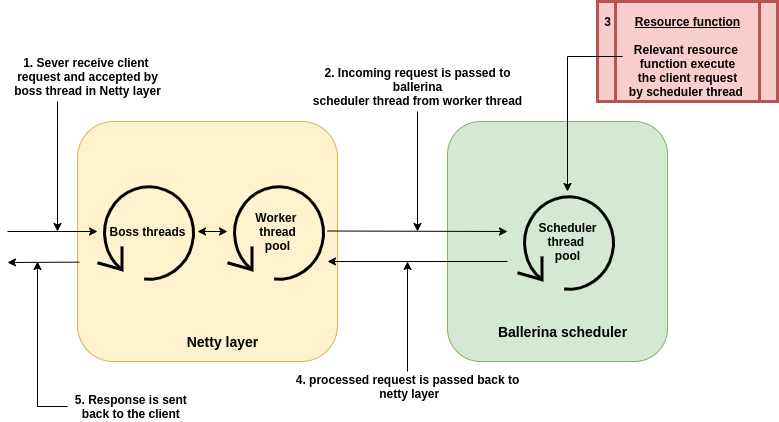
\includegraphics[scale=0.5]{figures/bal-internal.png}
	\end{center}
	\caption{Ballerina's internal architecture}
	\label{bal_internal}
\end{figure}

\section{Design steps}

The initial idea is coupled with the bound type of the program (CPU bound and IO-bound). Objectives were, (1) for a given Ballerina program identify its bound type, then (2) switch the server architecture which best suits the bound type. To determine the best server architecture, experiments are conducted. Following steps are taken to conduct the experiments. The below process is iterative.

\begin{itemize}
	\item Implement server architectures
	\item Use existing benchmark programs and implement new programs as necessary which have CPU intensive task and IO intensive tasks.
	\item Examine results.
	\item Debug and fine tune architectures based on results.
\end{itemize} 

\subsection{Testing process}

Each testing program is hosted as HTTP endpoints. Calling that endpoint invokes the relevant program. Jmeter act as a HTTP client. A typical web server is able to process concurrent HTTP requests. Jmeter can be configured to model this behavior. Jmeter continuously calls the given endpoint for a certain period under given configurations such as concurrency level. Then the following metrics are recorded,

\begin{itemize}
	\item Average latency — client HTTP requests are continuously sent to the web server and measure response time of each request. Then average is calculated.
	\item Standard deviation of latency — Standard deviation of above latency results.
	\item Throughput — Number of successful responses received per second.
	\item Error rate - Number of erroneous request as percentage of all request sent.
	\item Median, 75th percentile, 99th percentile of latency results.
\end{itemize} 

Then the performance is evaluated using above metrics. As an example when average latency is low and throughput is high for a given endpoint, that architecture's performance is good relative to others.
  

\begin{figure}[htbp]
	\begin{center}
		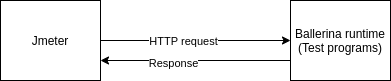
\includegraphics[scale=0.5]{figures/jmeter_bal.png}
	\end{center}
	\caption{Jmeter and Ballerina run time}
	\label{jmeter_testing}
\end{figure}



\subsection{Phase I - Implement and evaluate performance of different server architectures}

In this phase following server architectures are implemented. 

 \begin{itemize}
 	\item Original Ballerina architecture
 	\item Netty OIO
 	\item Removed Ballerina scheduler thread pool
 	\item Changing Ballerina scheduler thread pool size
 \end{itemize} 

The goal of implementing Netty OIO is to have a similar architecture of the thread per connection model. In this Netty's worker thread pool is configured to spawn a new thread per each client request. These threads block the execution until the task is finished. However, the Ballerina scheduler continues the execution in non-blocking fashion.

The expectation of removing the Ballerina scheduler is to inspect the behavior and performance when one thread pool is removed. The Netty layer's worker thread will carry out the execution of client tasks instead of the Ballerina scheduler thread. When there are multiple thread pools, it adds some overhead to the system. The expected behavior of removing thread pools is to improve the performance.  

Despite that, the purpose of having multiple thread pools is to avoid starvation where a task is keeping the thread pool busy so that another task is waiting and not getting a chance to execute for some time. Therefore that task is starved. instead of having a single thread pool for all functions, if other services have their own thread pool, then it is assured of having a certain number of threads at its disposal, hence it's not as sensitive to demands made by other services. The idea is when there are multiple thread pools, while one partition of the application is busy, but other parts of the application continue to work normally regardless of the rest of the system. This will add more stable characteristics to the system when the load is high.


%The multiple threadpools would require tuning to make sure each pool had enough threads and not too many. With a single threadpool you wouldn't need the tuning and might make better use of all the threads sometimes, but you might not have the predictability of knowing some important task would get the threads it needed to finish in a timely manner.
%

Finally, some variation to the number of threads in the Ballerina scheduler is performed. \textbf{Default thread pool size of Ballerina scheduler} is \textbf{$ \boldsymbol{2} \times \boldsymbol{Number\: of\: CPU\: cores}$}. Size of the thread pool is increased by \textbf{$ \boldsymbol{2} \times \boldsymbol{Number\: of\: CPU\: cores}$} and \textbf{$ \boldsymbol{4} \times \boldsymbol{Number\: of\: CPU\: cores}$}. In Ballerina connector calls such as database calls, block the execution thread. Increasing the number of threads can be beneficial in such situations because while other threads are blocking there are more threads to handle other tasks. 

For each architectural change, a number of benchmark programs were run which consist of CPU intensive and IO intensive features.
After conducting experiments with the above architectures, the following conclusions were made,

\begin{itemize}
	\item Netty OIO performance is worse in every situation — thus this architecture was no longer considered
	\item Removing Ballerina scheduler performs well for both IO and CPU intensive programs.
\end{itemize} 

Results and explanations are discussed in-depth in Chapter \ref{chap:5}. Based on these results, experiments were conducted with changing the size of the thread pool in the Ballerina scheduler.

\subsubsection{Test programs}

Following programs were implemented to evaluate the performance of each architectural change,

  \begin{itemize}
  	\item Check whether given number is prime - 3 primes are checked as prime small (521), prime medium(7919) and prime large(1000003)
  	\item Merge sort — 1000 random numbers are sorted
  	\item Read File from disk
  	\item Database test - Execute ‘select’ query on mysql database.
  \end{itemize} 
Above programs cover the CPU intensive cases and IO intensive cases. 

The sample result of a single experiment is shown in figure \ref{sample_result}. Four metrics (throughput, slandered divination, mean — average latency, 99th percentile  ) are shown in the plot. The X-axis represents the concurrent users. Y-axis represents the relevant metric.  

 \begin{figure}[htbp]
 	\begin{center}
 		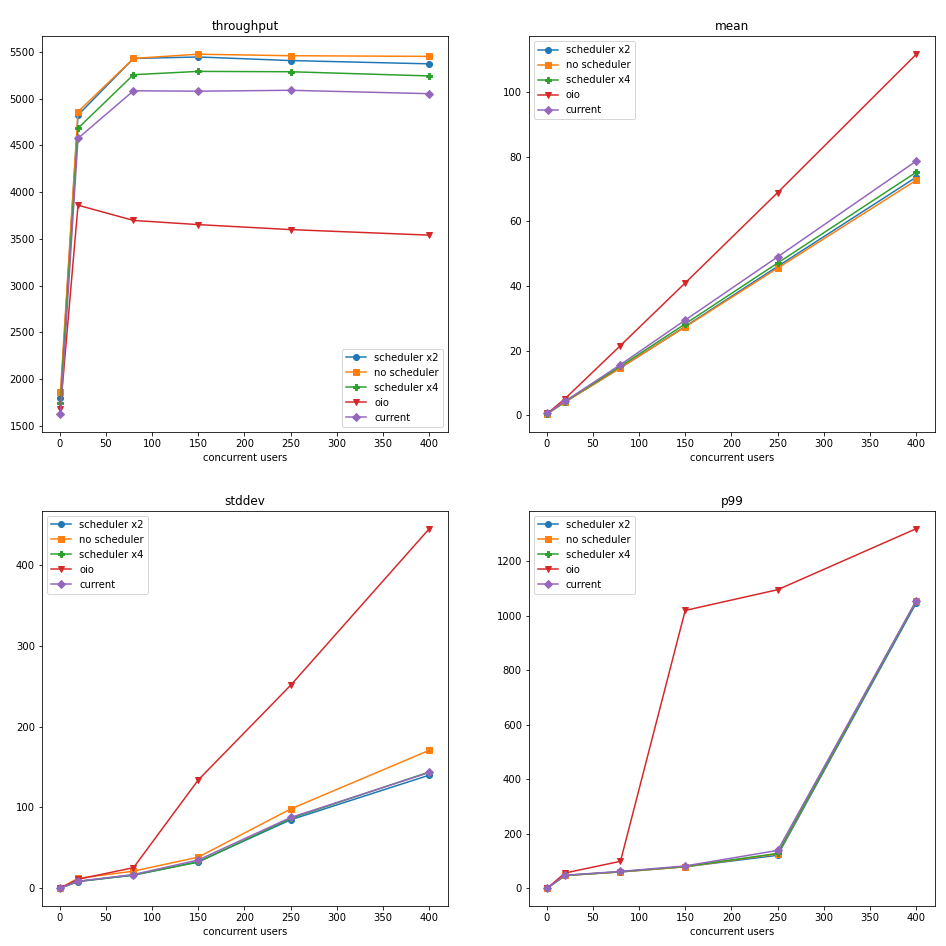
\includegraphics[scale=0.35]{figures/prime_small test results.png}
 	\end{center}
 	\caption{Sample experiment result}
 	\label{sample_result}
 \end{figure}

Then each metric is evaluated against each test program and each architectural change mentioned above.

\begin{comment}

\begin{table}[]
\begin{center}
\begin{tabular}{|l|l|l|l|l|l|}
\hline
Test case                                                     & \multicolumn{5}{l|}{Server architecture}                                                                                                                                                                                                                                \\ \hline
& \begin{tabular}[c]{@{}l@{}}Ballerina \\ original\end{tabular} & \begin{tabular}[c]{@{}l@{}}No \\ scheduler\end{tabular} & Netty OIO & \begin{tabular}[c]{@{}l@{}}Thread pool\\  size x 2\end{tabular} & \begin{tabular}[c]{@{}l@{}}Thread pool\\  size x 4\end{tabular} \\ \hline
\begin{tabular}[c]{@{}l@{}}Prime check \\ small\end{tabular}  &                                                               &                                                         &           &                                                                 &                                                                 \\ \hline
\begin{tabular}[c]{@{}l@{}}Prime check \\ medium\end{tabular} &                                                               &                                                         &           &                                                                 &                                                                 \\ \hline
\begin{tabular}[c]{@{}l@{}}Prime check \\ large\end{tabular}  &                                                               &                                                         &           &                                                                 &                                                                 \\ \hline
\begin{tabular}[c]{@{}l@{}}Database \\ call (IO)\end{tabular} &                                                               &                                                         &           &                                                                 &                                                                 \\ \hline
Merger sort                                                   &                                                               &                                                         &           &                                                                 &                                                                 \\ \hline
File read                                                     &                                                               &                                                         &           &                                                                 &                                                                 \\ \hline
\end{tabular}
\end{center}
\caption{Architecture comparison metric}
\label{tab:result_metric}
\end{table}

\end{comment}


Architectural changes to existing Ballerina run time involved extensive debugging because bugs in the implementation may incur wrong results. Therefore, this phase is conducted in an iterative manner to verify the results.
At the end of this stage, no architecture was performed well for IO use cases rather than CPU intensive cases and vice versa. Although changing thread pool size in the Ballerina scheduler started to show some significant results. Increasing thread pool size was affected differently in IO use cases. Then phase 2 is designed to analyze the variation of thread pool comprehensively.



\subsection{Phase II - Tuning thread pool size}

Thread pool tuning can be approached in two ways, \textbf{(1) White box system} — This requires complex mathematical modeling with queuing theories \cite{math_aproach_thread_pool_tuning}. Also, assumptions made at the beginning make it difficult to apply those modeling techniques for practical scenarios. \textbf{(2) Black box system} — In this approach, the thread pool system is considered as a black box where in-depth analysis of the thread pool system is not performed. Experiments are performed heuristically by changing parameters such as the size of the thread pool. Figure \ref{black_box_boundary} shows the boundary of the black box.
 
\begin{figure}[htbp]
	\begin{center}
		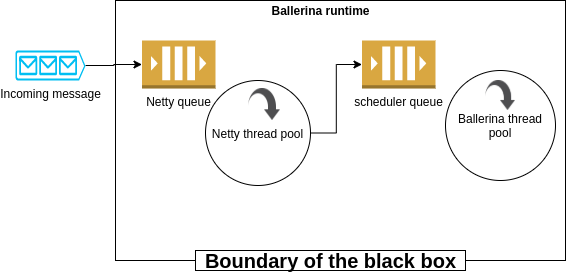
\includegraphics[scale=0.5]{figures/black_box_boundary.png}
	\end{center}
	\caption{Boundary of the black box}
	\label{black_box_boundary}
\end{figure}


This phase is preceded by considering the system as the black box. This model allows executing different programs under different sizes of the thread pool. Following the first phase of experiments, it is identified that changing thread pool size is affected differently for programs that consist of IO features. In the previous phase, experiments are conducted under different concurrency levels, but in this phase, fixed concurrency level is selected. Concurrency level was selected where a number near the point in the throughput curve which curve is starting to get flatten.

New sets of programs are implemented referring to multiple sources \cite{Ballerina_Performance,Ballerina_Website} in order to support programs that have rich IO call variations. In addition to the database calls in previous phase programs which have remote HTTP calls, GRPC calls and loops that contain these features are implemented. Subsection \ref{sub:phase3} provide more information. CPU intensive programs are no longer considered since it is difficult to extract CPU intensive operations directly by parsing AST. A more IO-oriented approach is used where the AST parser able to extract this information directly from the source code.  
	
\subsubsection{Experimental design} 

As a primary metric of evaluation average latency is used. Then each program is run under different thread pool sizes. Afterward, metrics are recorded. Table \ref{tab:pool_size_latency} shows summary of the results. Empty cells represent the average latency. Minimum latency values provide the optimal thread pool size for a given program. Instead of declaring thread pool size as a multiplier of the number of CPUs, explicit numbering is used for in-depth analysis of every thread pool size from 1 to 22. This range is selected because latency is always getting higher when increasing the number further.    

\begin{table}[]
	\caption{Program vs. Thread pool size - Latency results }
	\subcaption{The propose of this tabele is providing the insight of how data is gahtherd. Eplicit values are not presented here. Rsults section plots exact values }
	\begin{center}
	\begin{tabular}{|l|l|l|l|l|l|l|}
		\hline
		Program    & \multicolumn{6}{l|}{Pool size}        \\ \hline
		& 1            & 2 & 3 & ... & 19 & ... \\ \hline
		Program 1  & Ave. latency    & ...  & ...  & ...  &... &     \\ \hline
		Program 2  &      ...        & ...  & ...  & ...  &... &     \\ \hline
		Program 3  &      ...        & ...  & ...  & ...  &... &     \\ \hline
		...        &      ...        & ...  & ...  & ...  &... &     \\ \hline
		Program 50 &      ...        & ...  & ...  & ...  &... &     \\ \hline
		...        &      ...        & ...  & ...  & ...  &... &     \\ \hline
	\end{tabular}
	\end{center}
	\label{tab:pool_size_latency}
\end{table}

\subsection{Phase III - Building machine learning model to predict optimal thread pool size for given program}\label{sub:phase3}

At first, two models are considered in addition to predicting optimal thread pool. One model directly predicts the latency with given program features and given thread pool size. This model can be expressed as following function. 

$$ Latency \:(ms) = f(\:Program\:features,\:Threadpool\:size\:)$$

The weakness of this model is it heavily depends on the nature of the IO call. As an example latency is dependent on where the database is hosted if the given program has a database call. Also, latency is affected by the network connection also. Then the generalization of the result is very difficult.

The next model predicts optimal thread pool size for the given program. That model can be expressed as follows. That is the hypothesis that tries to resolve using a machine learning model. 

$$ Optimal\:thread\:pool\:size = f(\:Program\:features)$$

In order to build this model it is required find the minimum thread pool value from the result obtained by Design phase II. This step can be depicted as in figure \ref{optimal_pool_size}

\begin{figure}[htbp]
	\begin{center}
		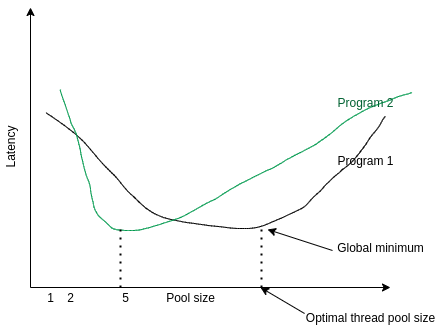
\includegraphics[scale=0.5]{figures/optimal_pool_size.png}
	\end{center}
	\caption{Obtaining optimal thread pool size}
	\label{optimal_pool_size}
\end{figure}

After some feature engineering steps, Features in table \ref{tab:programming-features}  are selected to train the machine learning model. Hyper parameters of each machine learning model are tuned for better accuracy. The implementation of hyper parameter tuning is presented in chapter \ref{chap:4}.

\begin{table}[]
	\caption{Programming features selected for machine learning model}
	\label{tab:programming-features}
	\begin{tabular}{|l|l|}
		\hline
		& Feature                                                      \\ \hline
		F1 & Number of HTTP connector calls                               \\ \hline
		F2 & Number of Database connector calls                           \\ \hline
		F3 & Number of non-blocking gRPC connector calls                  \\ \hline
		F4 & Number of loops containing HTTP connector calls              \\ \hline
		F5 & Number of loops containing Database connector calls          \\ \hline
		F6 & Number of loops containing non-blocking gRPC connector calls \\ \hline
	\end{tabular}
\end{table}

Then a training data set is created where input features are above programming features and output is optimal thread pool size. Table \ref{tab:data_frame} shows the shape of the data frame.


	\begin{table}[]
		\caption{Data frame shape of the training data set }
		\label{tab:data_frame}
		\begin{center}
		\begin{tabular}{|l|l|l|l|l|l|}
			\hline
			\multirow{2}{*}{Program} & \multicolumn{4}{l|}{Features} & \begin{tabular}[c]{@{}l@{}}Optimal Thread pool\\  size\end{tabular} \\ \cline{2-6} 
			& F 1    & F2    & ..    & Fn   &                                                             \\ \hline
			Program 1                &  ...  &  ...     &   ...    &  ...   &       n1                              \\ \hline
			...                      &  ...  &  ...     &   ...    &  ...   &       n2                              \\ \hline
		\end{tabular}
	\end{center}
		
	\end{table}

Then following machine learning models are selected and evaluated the accuracy of each model.

\begin{itemize}
	
	\item XGBoost
	\item Support Vector Machine
	\item Decision Tree
	\item Random Forest
	
\end{itemize}

For regression models \acrfull{MAPE} and \acrfull{MSE} are evaluated. For classification models F1 score and accuracy are evaluated.

The problem is originally a regression problem because the output of the model is a quantity (thread pool size). As this research provides a proof of concept, the problem is formulated as a classification model as well. Mapping the problem into a classification is possible because, as in the results of optimal thread pool sizes, clear clusters are visible. Chapter \ref{chap:5} provide results. Moreover, the distribution of the optimal thread pool is not uniform and only has several values.

\subsection{Phase IV - Parsing Ballerina AST to obtain features}\label{phase_iv}

First off, it is better to have some idea about what is \acrfull{AST}. It is a tree representation of the stricture of the source code.AST does not include all the details such as semicolon, parenthesis, etc. AST is used in semantic analysis of a code during the compilation process. Traversal of the AST verifies the correctness of the program against rules provided for that language. Moreover, information of the code can be extracted by traversing the AST.  Example of an AST is shown in figure \ref{AST_example} for code segment shown in figure \ref{code_for_ast}.

\begin{figure}[htbp]
	\begin{center}
		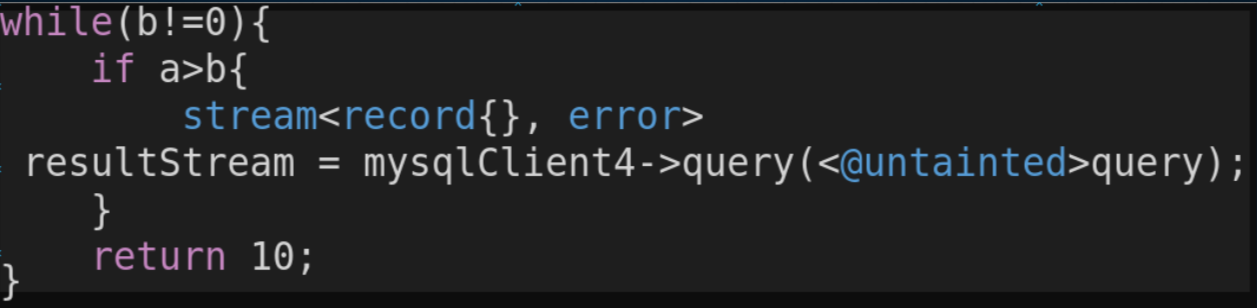
\includegraphics[scale=0.3]{figures/sample_code_for_ast.png}
	\end{center}
	\caption{Ballerina code}
	\label{code_for_ast}
\end{figure}

\begin{figure}[htbp]
	\begin{center}
		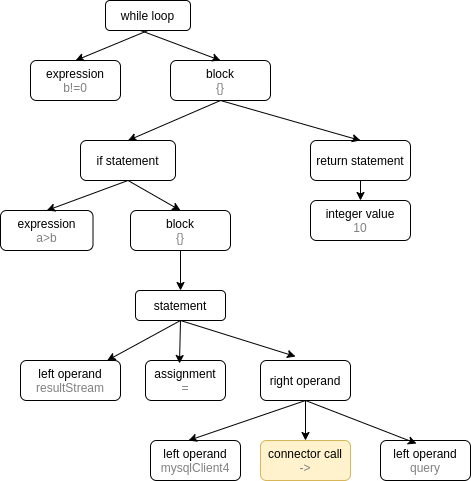
\includegraphics[scale=0.5]{figures/AST example.png}
	\end{center}
	\caption{Example AST}
	\label{AST_example}
\end{figure}

In this phase, a module is designed to parse Ballerina source code to feed the features into a machine learning model. Manual feature extraction is erroneous and harder when programs are large. First, this module accepts the Ballerina source code and output the array of features which is fed to the machine learning model. This is where Ballerina specific features are used that other languages are lack. 
Services are first-order functions in the Ballerina language. Then it is able to decide that the given program contains a web service. Then the subsequent parsing happens inside these service definitions. Also, network calls are part of the language. In the other languages, they are mostly library calls which is difficult to identify the given line of code that contains a network call. In Ballerina this is called a connector call. Recalling section \ref{Sec_Ballerina}, other languages provide network operations as library functions. If we try to extract such features from other languages, we need to know exactly which function call does an IO operation. In Ballerina, it is possible because connector calls can be differentiated naively. Algorithm 1 is implemented to extract features.

\begin{algorithm} \label{alg:ast_parser}
	
	\SetAlgoLined
	\KwIn{Source code (Ballerina.toml) }
	\KwOut{Feature Array}
	Start parsing\;
	
	\While{End program}{
		
		Traverse node\;{
			\If{Right Arrow Found}{
				
				\If{Left operand is Kind(Database call)}
				{
					\While{Backtrack}{
						
						\If{Loop start found}{
							Update feature array (Database call inside loop + 1)\;
							Stop backtracking and continue parsing\;
						}
						
						Update feature array (Direct Database call + 1)\;
						Continue parsing\;
					}
					
				}
			
				\If{left operand is Kind(Http call)}
				{
					\While{Backtrack}{
						
						\If{Loop start found}{
							Update feature array (HTTP call inside loop + 1)\;
							Stop backtracking and continue parsing\;
						}
						
						Update feature array (Direct HTTP call + 1)\;
						Continue parsing\;
					}
					
				}
			
				\If{left operand is Kind(GRPC-non-blocking call)}
				{
					\While{Backtrack}{
						
						\If{Loop start found}{
							Update feature array (GRPC call inside loop + 1)\;
							Stop backtracking and continue parsing\;
						}
						
						Update feature array (Direct GRPC call + 1)\;
						Continue parsing\;
					}
					
				}
				
			}
		}
		
			
	}
	
	\caption{Extract features using Ballerina AST}
\end{algorithm}

\section{Final design}\label{sec:final_design}

Finally, combing the above design steps, the overall design of the research is shown in figure \ref{hl_architecture}. First off, the Model is trained by different program features. In the second step trained machine learning model is produced. Then the model is given a new Ballerina source file. Program features are automatically extracted by AST parser. Then model output the optimal thread pool size for that given program. Then the program can be compiled with the suggested thread pool size. 

\section{Limitations}

There are several limitations that can be reorganized in the design. In design phase II, a fixed concurrency level is chosen. It is not explored how different concurrency levels are affected to the results. Another limitation is that hardware variable such as the number of CPUs, memory are not considered when constructing the hypothesis. Finally, when constructing the machine learning model it is only considered IO features. CPU extensive programs cannot be identified by parsing the source code. More explanations of these limitations are presented in chapter \ref{chap:6}.


\chapter{Implementation} \label{chap:4}

This chapter explains the steps taken to implement the research design and how the issues have been addressed occurred during implementation. Implementation can be divided into the following sub-topics.


\begin{itemize}
	\item Implementing server architectures in Ballerina
	\item Implementing test cases for performance evaluation
	\item Designing automated pipeline to obtain results
	\item Creating Machine learning models to classify programs
	\item Implementing AST parser.
\end{itemize}

\section{Implementing server architectures in Ballerina}

Ballerina source code written Java and Ballerina itself.

This involves deeper analysis existing Ballerina run time. Ballerina has three main non-blocking thread pools. One thread pool (Worker thread) lies in the scheduler. Other two thread pools lies in the Netty layer. Ballerina's internal architecture is explained in-detail in chapter 3. Initial step is making Netty thread pool to have blocking IO.
The Netty layer integrated as separate library (trasport-http)\cite{transport-http}. Following code fragment shows the implemented changes.  \textit{workerGroup = new OioEventLoopGroup(200000);} specify the use of blocking thread in the tread pool and allowing up to 20,000 threads in the thread pool. This thread pool hand over the client workload to Ballerina Scheduler. Following implementation is done in the Ballerina run-time.

\begin{lstlisting}[language=Java]

	public class DefaultHttpWsConnectorFactory implements HttpWsConnectorFactory {
	
	private final EventLoopGroup bossGroup;
	private final EventLoopGroup workerGroup;
	private final EventLoopGroup clientGroup;
	private EventExecutorGroup pipeliningGroup;
	
	private final ChannelGroup allChannels = new DefaultChannelGroup(GlobalEventExecutor.INSTANCE);
	
	public DefaultHttpWsConnectorFactory(int serverSocketThreads, int childSocketThreads, int clientThreads) {
	bossGroup = new OioEventLoopGroup(4);
	workerGroup = new OioEventLoopGroup(200000);
	clientGroup = new NioEventLoopGroup(clientThreads);
	}
	
	...
\end{lstlisting}


The next architectural change is \textbf{remove Ballerina scheduler} and use only Netty threads to complete client requests. Then the Ballerina scheduler is not involved in executing the client request. Normal procedure is incoming request is handed over to scheduler thread pool. Then scheduler thread pool completes the execution using its own threads and again handed over to the Netty layer to send the client response. 

This implementation should be carried out carefully. If the implementation is erroneous or having bugs, it would produce wrong results. Thus extensive debugging was used while implementation. This was difficult due to the tight coupling of the Netty layer and Ballerina scheduler. In order to implement that I created separate \textbf{Task Executor} as \textit{MyExecutor}. Execution of client requests is defined in that java Class. The \textit{submit()} method accept the incoming request and execute the instructions using the incoming thread which is proceeded from the Netty thread pool.


\begin{lstlisting}[language=Java]

public class BallerinaHTTPConnectorListener implements HttpConnectorListener {
...

@Override
public void onMessage(HttpCarbonMessage inboundMessage) {

...

MyExecutor.submit( service, httpResource.getName(), callback, properties, signatureParams);

...

\end{lstlisting}


In addition to major architectural changes, fine-tuning to implemented architecture and existing architecture is carried out continuously. Those fine-tune assisted to narrow down to research to thread pool optimization. In the final phase, existing Ballerina architecture is selected and tested with different thread pool numbers. A number of threads in the thread pool is set through the environment variable. The following code snippet shows that.


\begin{lstlisting}[language=Java]
public class Scheduler {
 ...

// Setting Ballerina thread pool size 
private static String poolSizeConf = System.getenv(BLangConstants.BALLERINA_MAX_POOL_SIZE_ENV_VAR);

...

public Scheduler(boolean immortal) {
	try {
 		if (poolSizeConf != null) {
  			poolSize = Integer.parseInt(poolSizeConf);
 		}
	} catch (Throwable t) {
	
		// Log and continue with default
		err.println("ballerina: error occurred in scheduler while reading system variable:" +
		BLangConstants.BALLERINA_MAX_POOL_SIZE_ENV_VAR + ", " + t.getMessage());
	}
	this.numThreads = poolSize;
	this.immortal = immortal;

	console.println("Pool size: "+poolSize);
}

\end{lstlisting}



\section{Implementing test cases for performance evaluation}

Test cases were implemented in Ballerina language. This implementation is very crucial since all the results depend on the designing of test programs. In the initial phases, all the test programs are designed to have IO calls and CPU-intensive instructions. Some of the test cases were designed by the Ballerina team \cite{Ballerina_Performance} which was originally designed to evaluate the performance of Ballerina run time. Those tests included external service calls (HTTP requests). This study able to re-use them and reproduce the results.

Since Ballerina is a service-oriented language implementation is well structured. In Ballerina a service is packed into a single unit. The following example represents the service called \textit{myservice}. That service is exposed outside via port number 9090. All the relevant implementation to this service goes inside the braces. There can be multiple services exposed via different ports. The structure of this is well suited with micro-service architecture \cite{nadareishvili2016microservice}.


\begin{lstlisting}[language=Java]
 service myservice on new http:Listener(9090) {
	
	}

\end{lstlisting}

Inside a service, it can be implemented resource function. A single resource function can be considered as a single endpoint in RESTful API. Following resource function represent the endpoint \textit{http://hostname:9090/book/someBookId}

\begin{lstlisting}[language=Java]

service myservice on new http:Listener(9090) {


@http:ResourceConfig {
methods: ["GET"], path: "/book/{bookId}"
}
resource function getById(http:Caller caller, http:Request req, string bookId) {
	json? payload = booksMap[bookId];
	http:Response response = new;
	if (payload == null) {
		response.statusCode = 404;
		payload = "Item Not Found";
	}
	response.setJsonPayload(untaint payload);
	var result = caller->respond(response);
	if (result is error) {
	log:printError("Error sending response", err = result);
	}
}

\end{lstlisting}

Similar to the above resource function all the test cases are enclosed as resource functions. Then the test cases are invoked by HTTP request. The following code segment shows one test case used for testing. It includes a single blocking IO call ( Databse call). 

\begin{lstlisting} [language=Java]
resource function db_select(http:Caller caller, http:Request request) returns error? {
	http:Response response = new;
	var params = request.getQueryParams();
	var id = <string>params.get("id")[0];//<string>params.id
	var query = "SELECT * FROM emp where id = "+id;
	
	stream<record{}, error> resultStream = mysqlClient4->query(<@untainted>query);
	
	record {|record {} value;|}|error? result = resultStream.next();
	
	error? e = resultStream.close();
	
	response.setTextPayload(<@untainted> io:sprintf("%s", result));
	check caller->respond(response);
	
	}
\end{lstlisting}

Many programs similar to above are implemented to evaluate test cases.

\section{Designing automated pipeline to obtain results}

This section explains how the results were obtained and what actions were taken into account to ensure accuracy. 

A proper testing environment is very important since results may inaccurate without proper isolation. Testing environments are isolated with used Docker \cite{docker} containers. It minimizes the interference occurred by other processes. Also, it limits resource usage by specifying the upper bound. . 

Performance metrics are obtained primarily by Jmeter \cite{jmeter}. In order to minimize the instrumentation errors, results are validated with a load testing tool called Tsung \cite{tsung}.

\begin{figure}[htbp]
  \begin{center}
    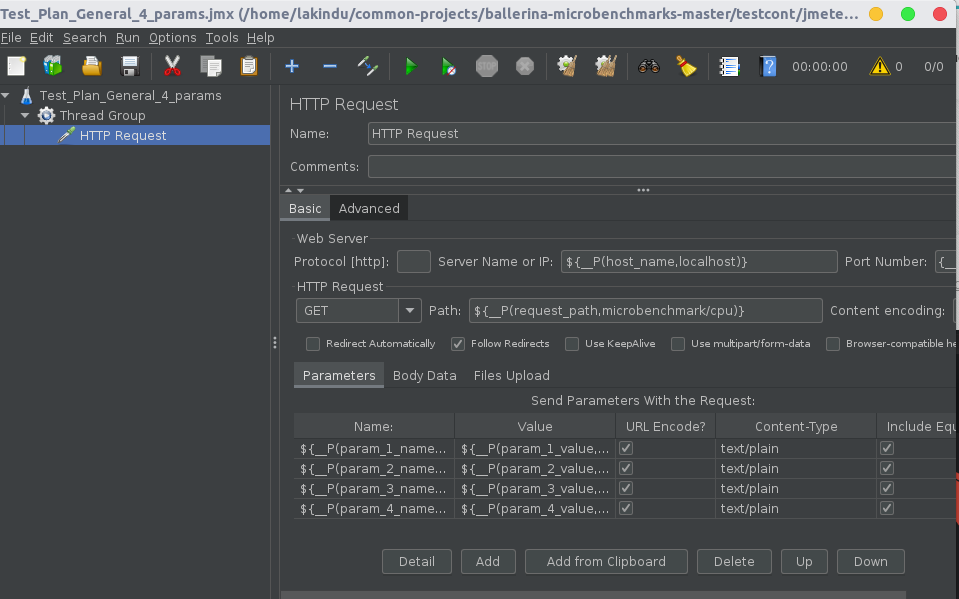
\includegraphics[scale=0.3]{figures/jmeter_sc.png}
    \end{center}
  \caption{Jmeter interface}
  \label{jmeter_ui}
\end{figure}


\begin{figure}[htbp]
	\begin{center}
		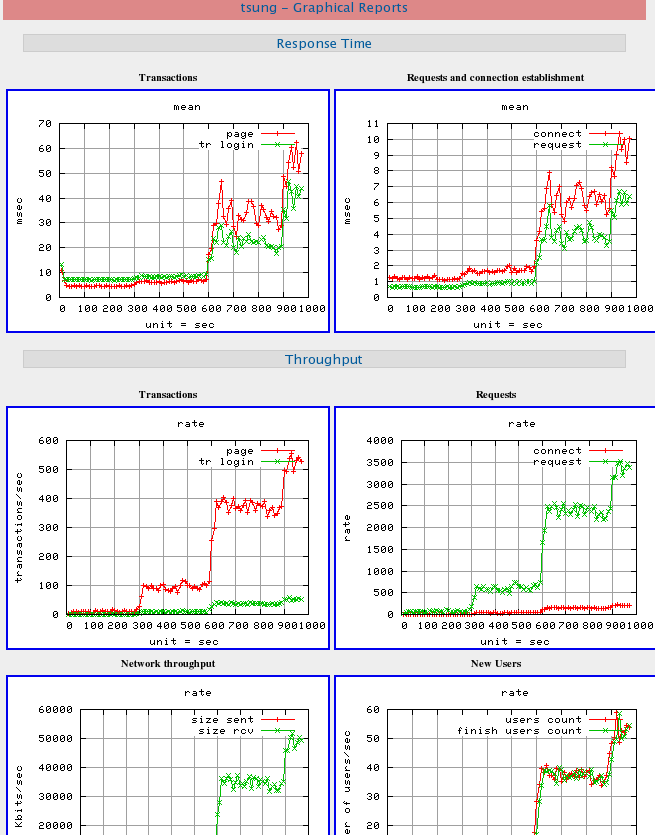
\includegraphics[scale=0.4]{figures/tsung-graph.png}
	\end{center}
	\caption{Tsung stat report}
	\label{tsung-graph}
\end{figure}


Jmeter has both command line and graphical user interface. Tsung configurations are only available with command-line and XML files. Configuring tests is easier in Jmeter than Tsung. Thus Tsung is only used to validate the results in early phases.  Several tests are executed using both tools and obtained the latency results to validate the tools. Some results are shown in table \ref{jmeter_and_tsung}. Average variance is \textit{0.29 ms}.

\begin{table}[htbp]
	\caption{Latency results comparison using Jmeter and Tsung}
	\label{jmeter_and_tsung}
	\begin{center}
	\begin{tabular}{|l|l|l|l|}
		\hline
		Test   & Jmeter  & Tsung   & Description                                                                               \\ \hline
		test 1 & 27.42ms & 24.71ms & \begin{tabular}[c]{@{}l@{}}Database call - \\ concurrency level 80\end{tabular}           \\ \hline
		test 2 & 57.31ms & 57.22ms & \begin{tabular}[c]{@{}l@{}}External http call -\\ concurrency level 80\end{tabular}       \\ \hline
		test 3 & 44.97ms & 45.18ms & Merger sort - concurrency level 60                                                        \\ \hline
		test 4 & 34.76ms & 34.42ms & \begin{tabular}[c]{@{}l@{}}database call - \\ concurrency level 100\end{tabular}          \\ \hline
		test 5 & 28.44ms & 28.32ms & \begin{tabular}[c]{@{}l@{}}Prime number calculation -\\ concurrency level 80\end{tabular} \\ \hline
	\end{tabular}
	\end{center}

\end{table}


Testing pipeline is consited of two parts, which are,

\begin{enumerate}
	\item Ballerina run time where tests were implemented
	\item Jmeter/Tsung clients to measure the performance metrics 
\end{enumerate}
	
In addition to the above, a database server, an external HTTP server, and gRPC server are implemented to run tests. Figure \ref{testing_env} depicts the architecture of the testing environment. 3  \acrfull{VM} that are hosted in Google cloud is used. VM that running Ballerina run time and Jmeter client has 6 core CPU with 12 GB of memory. The other two VM are 2 core CPUs with 4 GB of memory. To eliminate bottlenecks of external services, CPU usage is monitored to keep the CPU usage under 80\% using Stack Driver scripts. Hence results only depend on Ballerina run time. Since Ballerina run time, Jmeter client and Database server is hosted in same VM using docker, Maximum CPU usage is limited to 2 cores per Jmeter and Ballerina run time. The database server is allocated with 1.2 CPU cores. With maximum concurrency level, the Database server used only average of 83\% of CPU. 

Continuous monitoring ensured no bottleneck due to resource limitations. The testing pipeline is automated since the duration of the test is very long. Some tests were running for days and failing a test at the middle of execution because of an error resulted running them again from begining. Implementation of the pipeline is included in code listings.

\begin{figure}[htbp]
	\begin{center}
		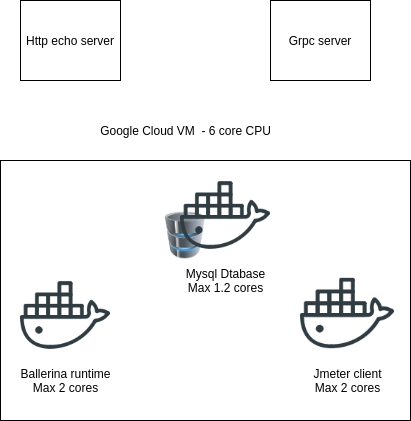
\includegraphics[scale=0.5]{figures/Tes_env.png}
	\end{center}
	\caption{Testing environment}
	\label{testing_env}
\end{figure}

\section{Creating Machine learning models to predict optimal thread pool size}

The final implementation of this research is building a machine learning model to predict the best architecture based on programming features. Based on early results, the research is narrowed down to find the optimal thread pool size instead of predicting architecture. The final model predicts the optimal thread pool size for a given program. Two approaches were used to obtain results. One way is making the problem a classification problem and the other is making it a regression problem. Then relevant metrics are compared to evaluate the best approach. Following machine learning models are implemented,
\begin{itemize}
	
	\item XGBoost
	\item Support Vector Machine
	\item Decision Tree
	\item Random Forest
	
\end{itemize}

Following code shows implementation of XGBoost regression model.

\begin{lstlisting} [language=Python]

from numpy import loadtxt
from xgboost import XGBRegressor
from sklearn.model_selection import train_test_split
from sklearn.metrics import accuracy_score
from sklearn.metrics import mean_absolute_percentage_error
from sklearn.metrics import mean_squared_error

def cross_validation_r(model,X,Y):

	cv = ShuffleSplit(n_splits=5, test_size=0.3, random_state=1)
	
	scores = cross_validate(model, X, Y, cv=cv , scoring=['neg_mean_squared_error','neg_mean_absolute_percentage_error'])
	
	
	cv_mape=scores['test_neg_mean_absolute_percentage_error']
	cv_mse=scores['test_neg_mean_squared_error']
	
	print("MAPEs: ",cv_mape)
	print("MSEs: ",cv_mse)
	
	print("MAPE: %0.2f%% with a standard deviation of %0.2f" % (abs(cv_mape.mean()*100), cv_mape.std()))
	print("MSE: %0.2f  with a standard deviation of %0.2f" % (abs(cv_mse.mean()), cv_mse.std()))
	
# load data
dataset = loadtxt('g_dataset_class_2.csv', delimiter=",")
# split data into X and y
X = dataset[:,0:5]
Y = dataset[:,6]
# split data into train and test sets
seed = 6
test_size = 0.3

X_train, X_test, y_train, y_test = train_test_split(X, Y, test_size=test_size, random_state=seed)
# fit model no training data
model = XGBRegressor()

model.fit(X_train, y_train)
# make predictions for test data
y_pred = model.predict(X_test)
predictions = [round(value) for value in y_pred]


# Cross validation
print("# cross validated evaluations")
print(cross_validation_r(model,X,Y))

# cross validated evaluations
MAPE: 7.92% with a standard deviation of 0.01
MSE: 1.46  with a standard deviation of 0.15

\end{lstlisting}


\subsection{Hyper parameter tuning}

Hyper-parameters are the properties that govern the entire training process. The output of the parameters was used when training each model. The following code shows that Random search hyperparameter tuning for the Decision tree model.

\begin{lstlisting} [language=Python]

def hyperparameter_tuning(tr_features, tr_labels):
	# Number of trees in random forest
	n_estimators = [int(x) for x in np.linspace(start = 200, stop = 2000, num = 1000)]
	# Number of features to consider at every split
	max_features = ['auto', 'sqrt']
	# Maximum number of levels in tree
	max_depth = [int(x) for x in np.linspace(5, 150, num = 50)]
	max_depth.append(None)
	# Minimum number of samples required to split a node
	min_samples_split = [x for x in range(1,51)]
	# Minimum number of samples required at each leaf node
	min_samples_leaf = [x for x in range(1,51)]
	# Method of selecting samples for training each tree
	bootstrap = [True, False]
	# Create the random grid
	random_grid = {
	'max_features': max_features,
	'max_depth': max_depth,
	'min_samples_split': min_samples_split,
	'min_samples_leaf': min_samples_leaf,
	}
	
	rf_hyper = tree.DecisionTreeRegressor()
	rf_random = model_selection.RandomizedSearchCV(estimator = rf_hyper, param_distributions = random_grid, n_iter = 100, cv = 3, verbose=2, random_state=42, n_jobs = -1)
	# Fit the random search model
	rf_random.fit(tr_features, tr_labels)
	return rf_random.best_params_
	
	a =hyperparameter_tuning(X_train,y_train)
	return a

\end{lstlisting}


\section{Conclusion}

This chapter presented some implementations used in each stage of the research. More implementations such as test programs, AST parser can be found in GitHub repositories mentioned in Appendix \ref{appendix:c}.

\chapter{Results and Evaluation}\label{chap:5}

This chapter compare the results obtained in each stage and how those results are supported to narrow down the research to find number of optimal thread pool for given program. In the early phases broader measurement metrics ( average latency, throughput, Standard deviation, average latency, Median latency, 99th percentile of latency, error rate ) were analyzed to compare  architectures. Some metrics  In later phases average latency (in milliseconds) is used as main metric to compare performance. Chapter 3 explains the these metrics in detail.

In the first phase following architectures were implemented,

\begin{itemize}
	\item Ballerina current architecture
	\item Increasing Ballerina scheduler thread pool size into 2 times and 4 times
	\item Removing Ballerina Scheduler thread pool
	\item Changing Netty layer worker thread pool as thread per connection model  (Netty \acrshort{OIO}) 
\end{itemize}

\section{Results comparison of different architectures}

\begin{figure}[htbp]
	\begin{center}
		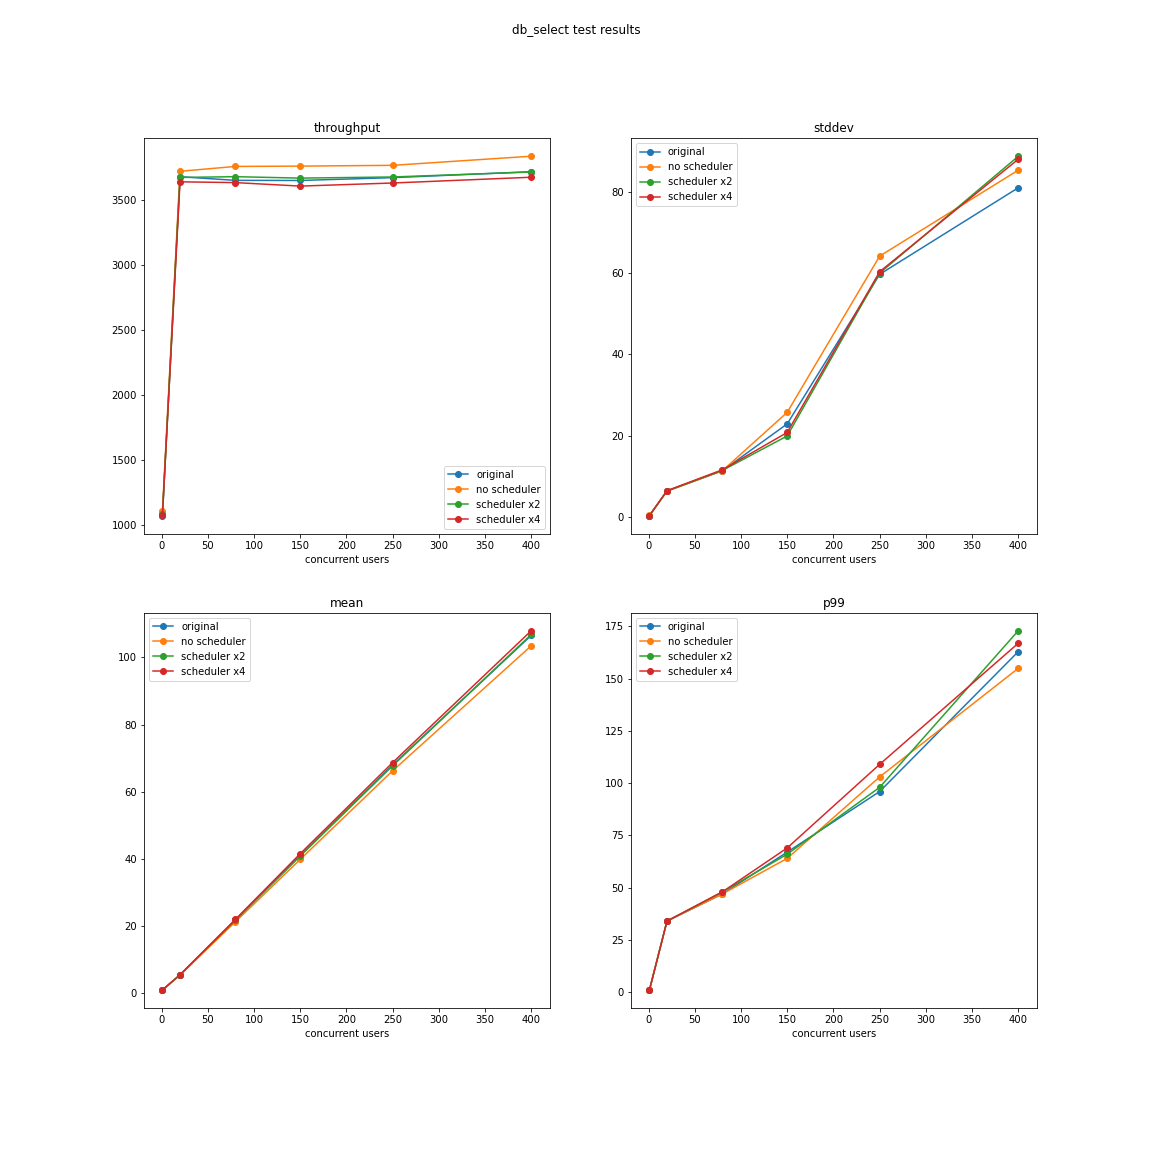
\includegraphics[scale=0.5]{figures/db_select test results.png}
	\end{center}
	\caption{Throughput, Avg. Latency(Mean), Standard deviation(stddev) and 99th percentile of latency  of Database call test for 1. Make twice the thread pool size of scheduler 2. Ballerina removing scheduler thread pool 3. Make 4 times the thread pool size of scheduler 4. Netty OIO architecture 5. Ballerina current architecture }
	\label{phase-1-database-all-architectures}
\end{figure}

\begin{figure}[htbp]
	\begin{center}
		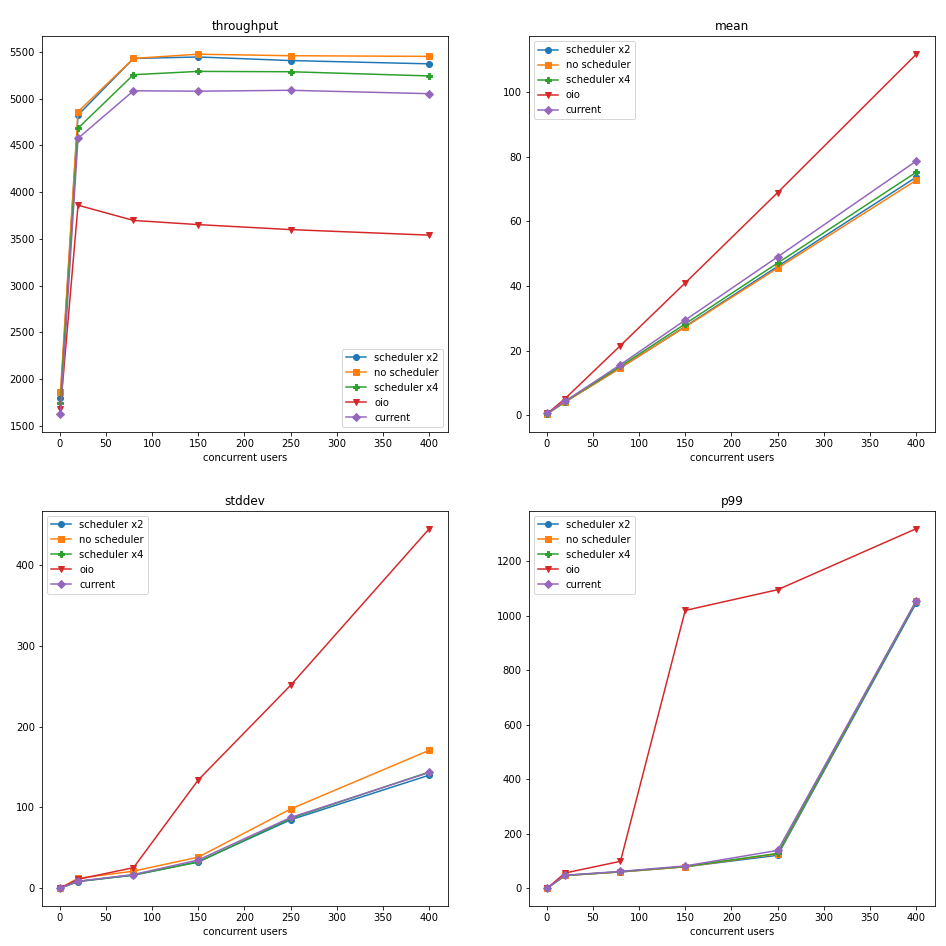
\includegraphics[scale=0.5]{figures/prime_small test results.png}
	\end{center}
	\caption{Throughput, Avg. Latency(Mean), Standard deviation(stddev) and 99th percentile of latency for Prime small test }
	\label{phase-1-prime-small-all-architectures}
\end{figure}

\begin{figure}[htbp]
	\begin{center}
		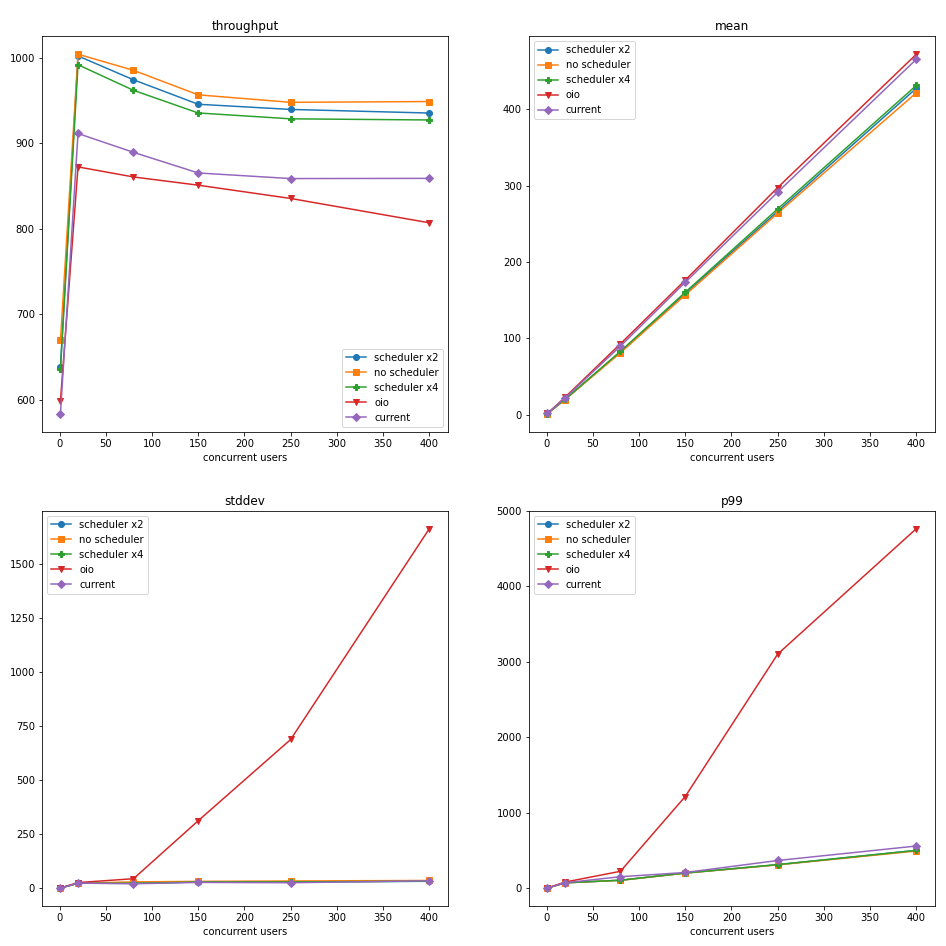
\includegraphics[scale=0.5]{figures/prime_medium test results.png}
	\end{center}
	\caption{Throughput, Avg. Latency(Mean), Standard deviation(stddev) and 99th percentile of latency for Prime medium test }
	\label{phase-1-prime-medium-all-architectures}
\end{figure}

\begin{figure}[htbp]
	\begin{center}
		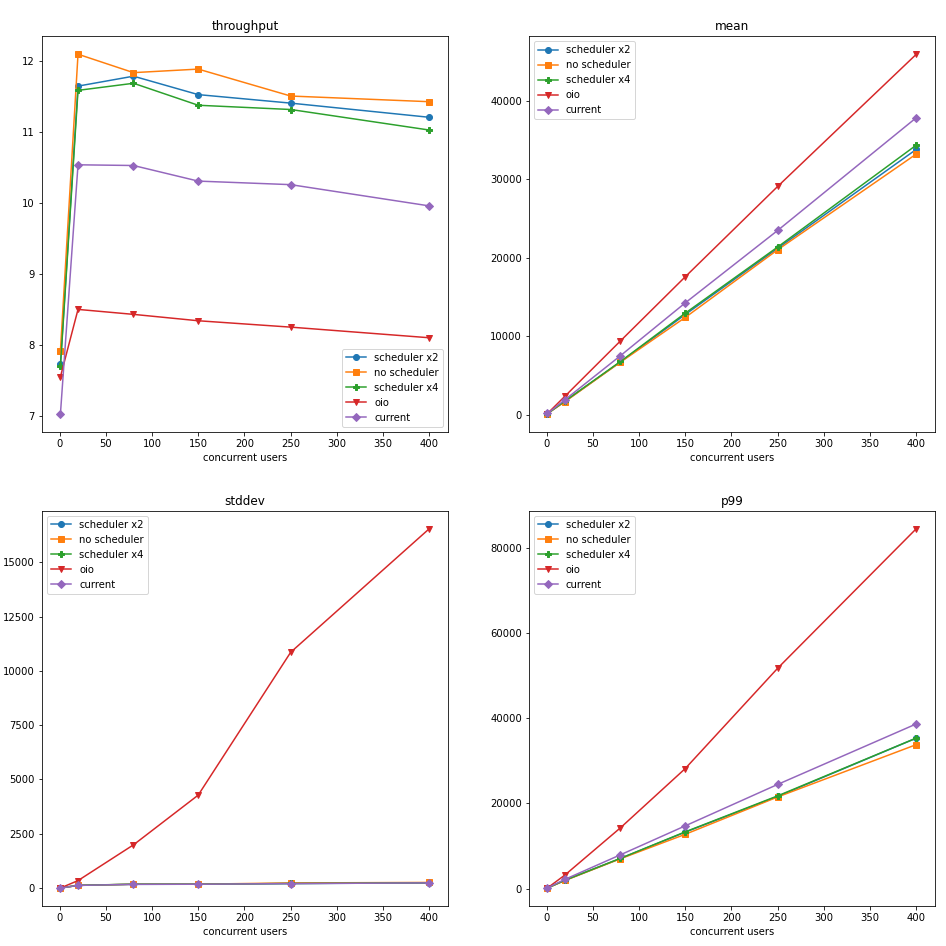
\includegraphics[scale=0.5]{figures/prime_large test results.png}
	\end{center}
	\caption{Throughput, Avg. Latency(Mean), Standard deviation(stddev) and 99th percentile of latency for prime large test }
	\label{phase-1-prime-large-all-architectures}
\end{figure}

\begin{figure}[htbp]
	\begin{center}
		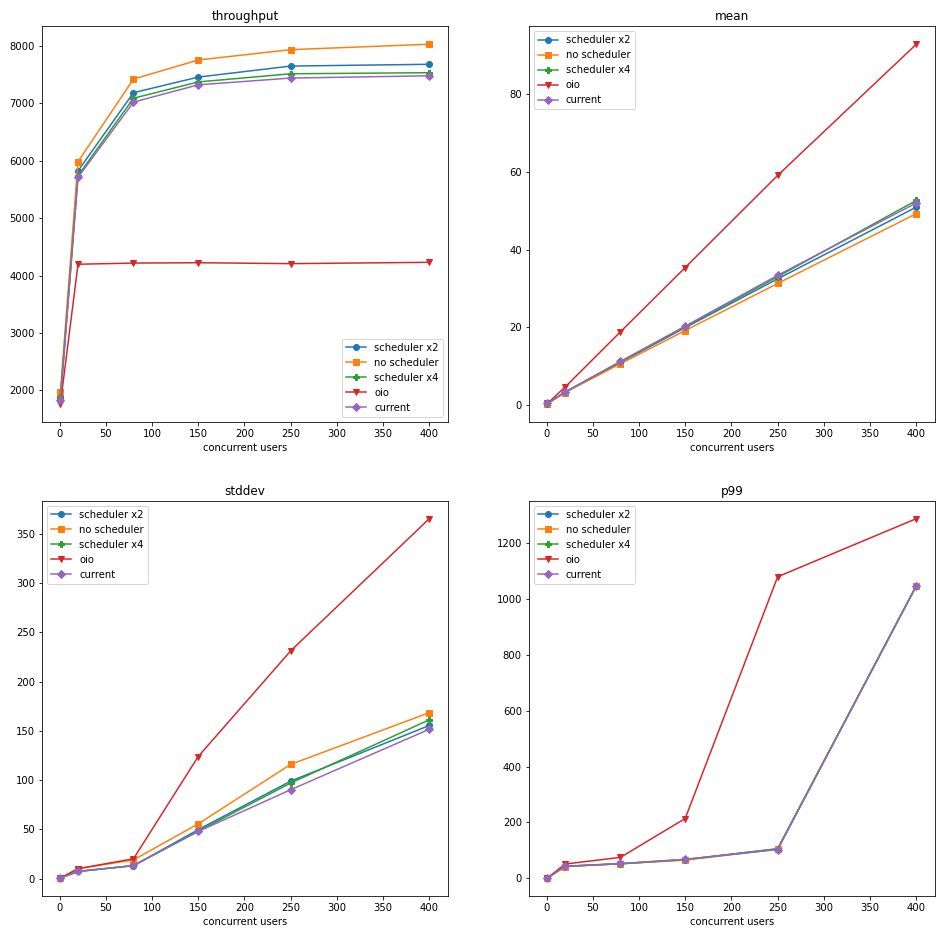
\includegraphics[scale=0.5]{figures/file test results.png}
	\end{center}
	\caption{Throughput, Avg. Latency(Mean), Standard deviation(stddev) and 99th percentile of latency for file read test  }
	\label{phase-1-file-read-all-architectures}
\end{figure}

Metrics such as error rate is not shown in the plots since those metrics are used to verify the validity of obtained results in intermediate steps. Performance tests were started with Current ballerina architecture, Removing ballerina scheduler thread pool and Netty OIO architecture. Since Netty OIO performance (High latency and low throughput) is lowest in every case, focus is moved to tread pools. Then the behavior is analyzed with adding more threads to scheduler thread pool. Figures \ref{phase-1-database-all-architectures},\ref{phase-1-prime-small-all-architectures},\ref{phase-1-prime-medium-all-architectures},\ref{phase-1-prime-large-all-architectures},\ref{phase-1-file-read-all-architectures}, shows the throughput and latency results for Database, Prime small,Prime medium,Prime large and File read. In mentioned graphs it can be seen that OIO architecture has the lowest throughput, the highest latency and higher standard deviation among all the other architectural changes for almost every concurrency level. After initial tests OIO architecture was not considered for future tests. 

Another significant indication that removing ballerina scheduler able to gain significant performance(Higher throughput and lower latency). That performance gain is independent form the program type. Thus,it was not possible to find distinct situations where a certain architecture would perform well for one program type while another architecture performs well for another program type. Although changing thread pool size affected differently in CPU bound(Prime test) and IO cases (Database test). Then the direction of server architecture tuning is focused on tread pool tuning. In this phase it is only changed two values of thread pool size. That is not sufficient to bring any conclusion.

\begin{figure}[htbp]
	\begin{center}
		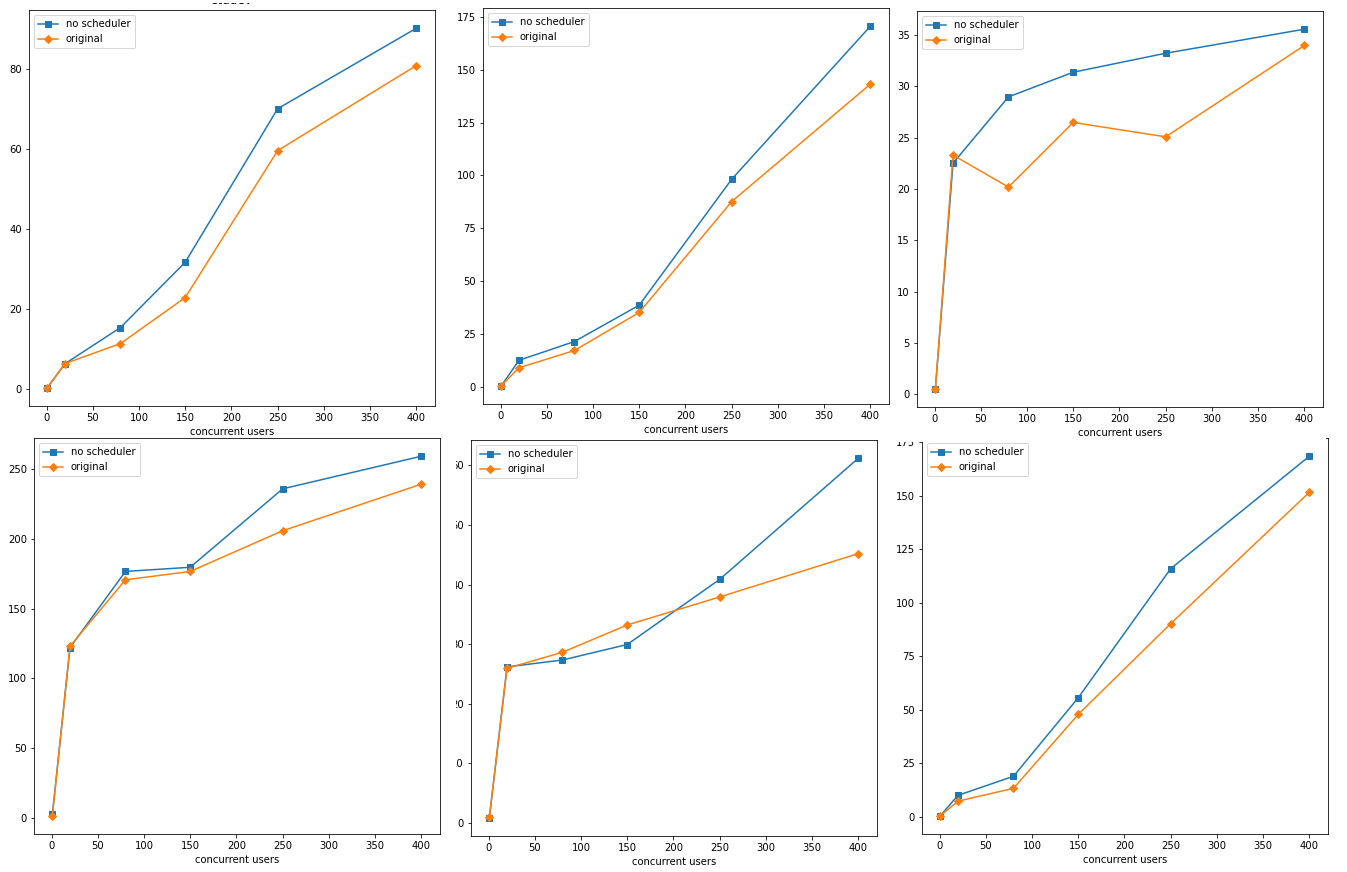
\includegraphics[scale=1.2]{figures/db-ps-pm-pl-ms-fr.png}
	\end{center}
	\caption{Standard deviation comparison of Database select test, Prime small test, Prime medium test, Prime large test, Prime medium test, Merge sort, File test }
	\label{all_sd}
\end{figure}


In order to evaluate the performance of sever architecture in depth standard deviation is another important metric. Although removing ballerina scheduler perform well by throughput and latency, standard deviation is higher than current ballerina architecture for every program type. Since OIO architecture has greater standard deviations, values are not clear in the above figures. To analyze more clearly Figure \ref{all_sd} shows standard deviation values for current architecture and removed scheduler architecture. It is clear that having Ballerina's scheduler thread pool provide more stable results. Also, it is noticeable that increasing thread pool size of the Ballerina scheduler thread pool able to decrease the average latency closer as removed Ballerina scheduler thread pool. There is a trade off between stability and latency when scheduler thread pool is removed. In order to maintain stability it is chosen to keep ballerina scheduler thread pool.

Test programs were designed to have CPU bound and IO bound features in order to evaluate which server architecture is better for IO bound programs and which architecture is better for CPU bound program. Results obtained in this phase does not able to differentiate performance of architecture based on program type. However, it is clear that changing the thread pool size affected differently in IO bound and CPU bound programs. When comparing the throughput of Database test case (Figure \ref{phase-1-database-all-architectures}) and Prime small test case (Figure \ref{phase-1-prime-small-all-architectures}), changing thread size affected most in the prime small test. In Database test, increasing thread pool size doesn't change the throughput and latency values significantly. The reason behind that scenario can be explained as, since database call is a blocking call which blocks the execution thread, thread pool size variation ( 2 times and 4 times the default scheduler thread pool size) is not sufficient to gain significant performance different. Next experiments results are based on introducing more thread pool sizes to the ballerina scheduler considering results on this phase. Also, there is lack of programs based on IO features in the initial experiments even though there are many CPU intensive programs. Thus new IO programs are added to the experiments.

\section{Results comparison of different thread pool size}

\begin{figure}[htbp]
	\begin{center}
		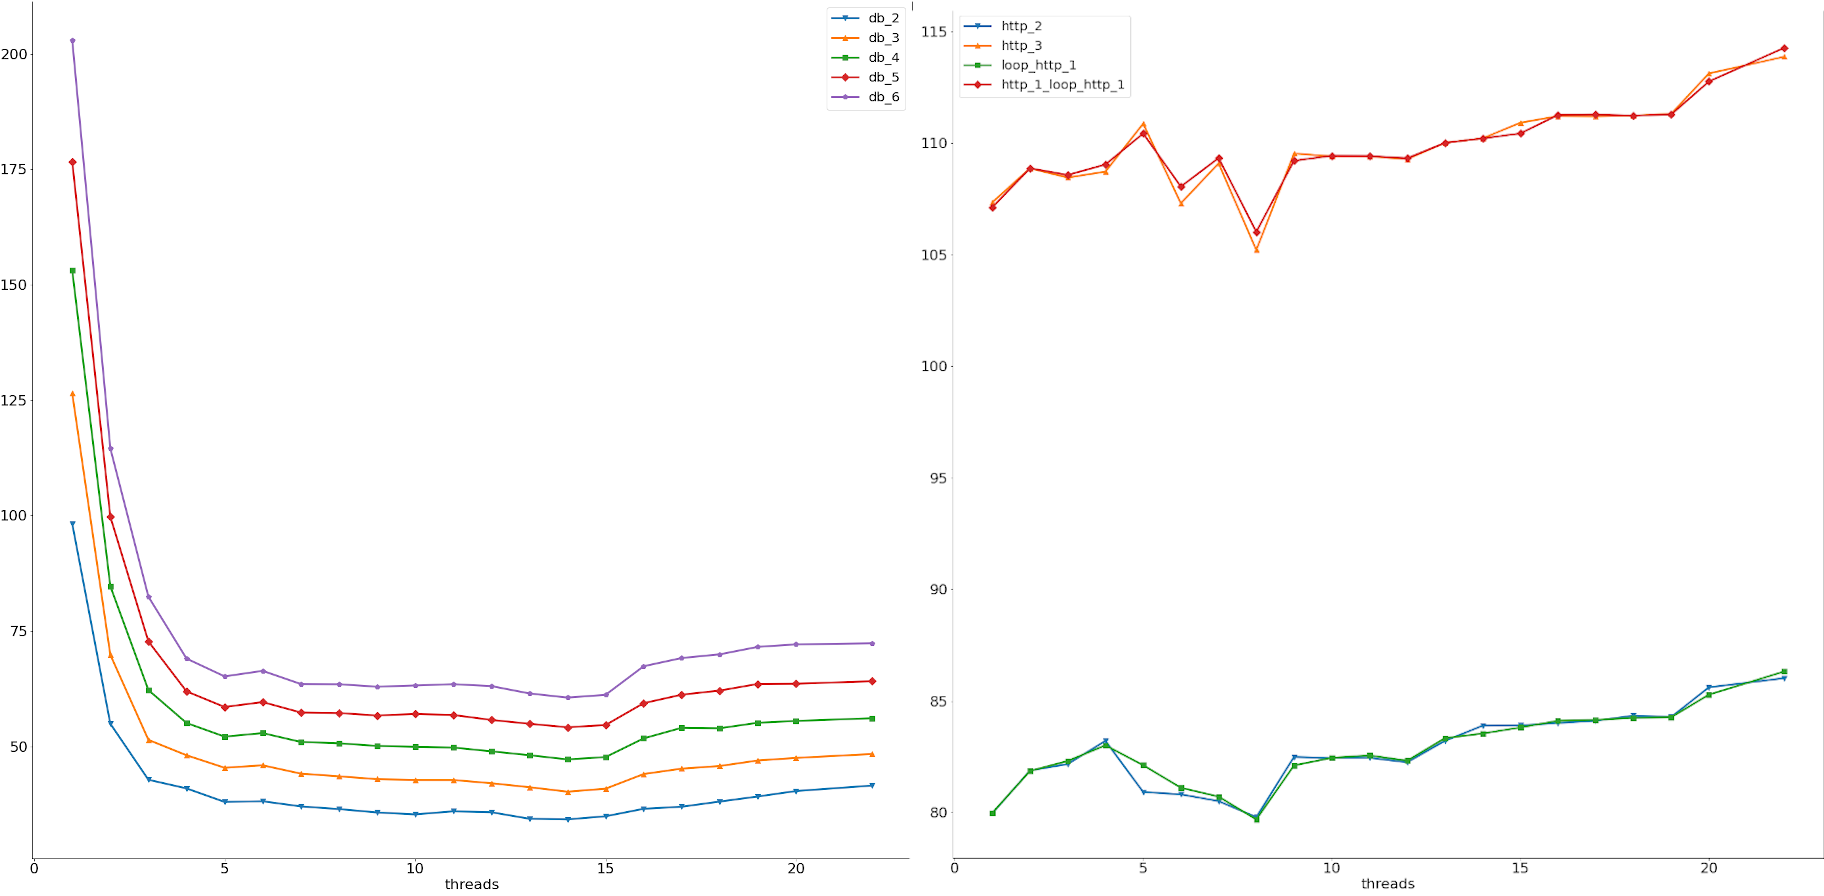
\includegraphics[scale=1]{figures/pool-db-http.png}
	\end{center}
	\caption{Left plot shows Thread pool size vs Average latency (millisecond) for number of database calls. \textbf{db\_2} represent program has 2 database calls. Right plot shows Thread pool size vs Average latency (millisecond) for number of http calls and number of loops which contains http calls}
	\label{thread_pool_database_and_http}
\end{figure}

\begin{figure}[htbp]
	\begin{center}
		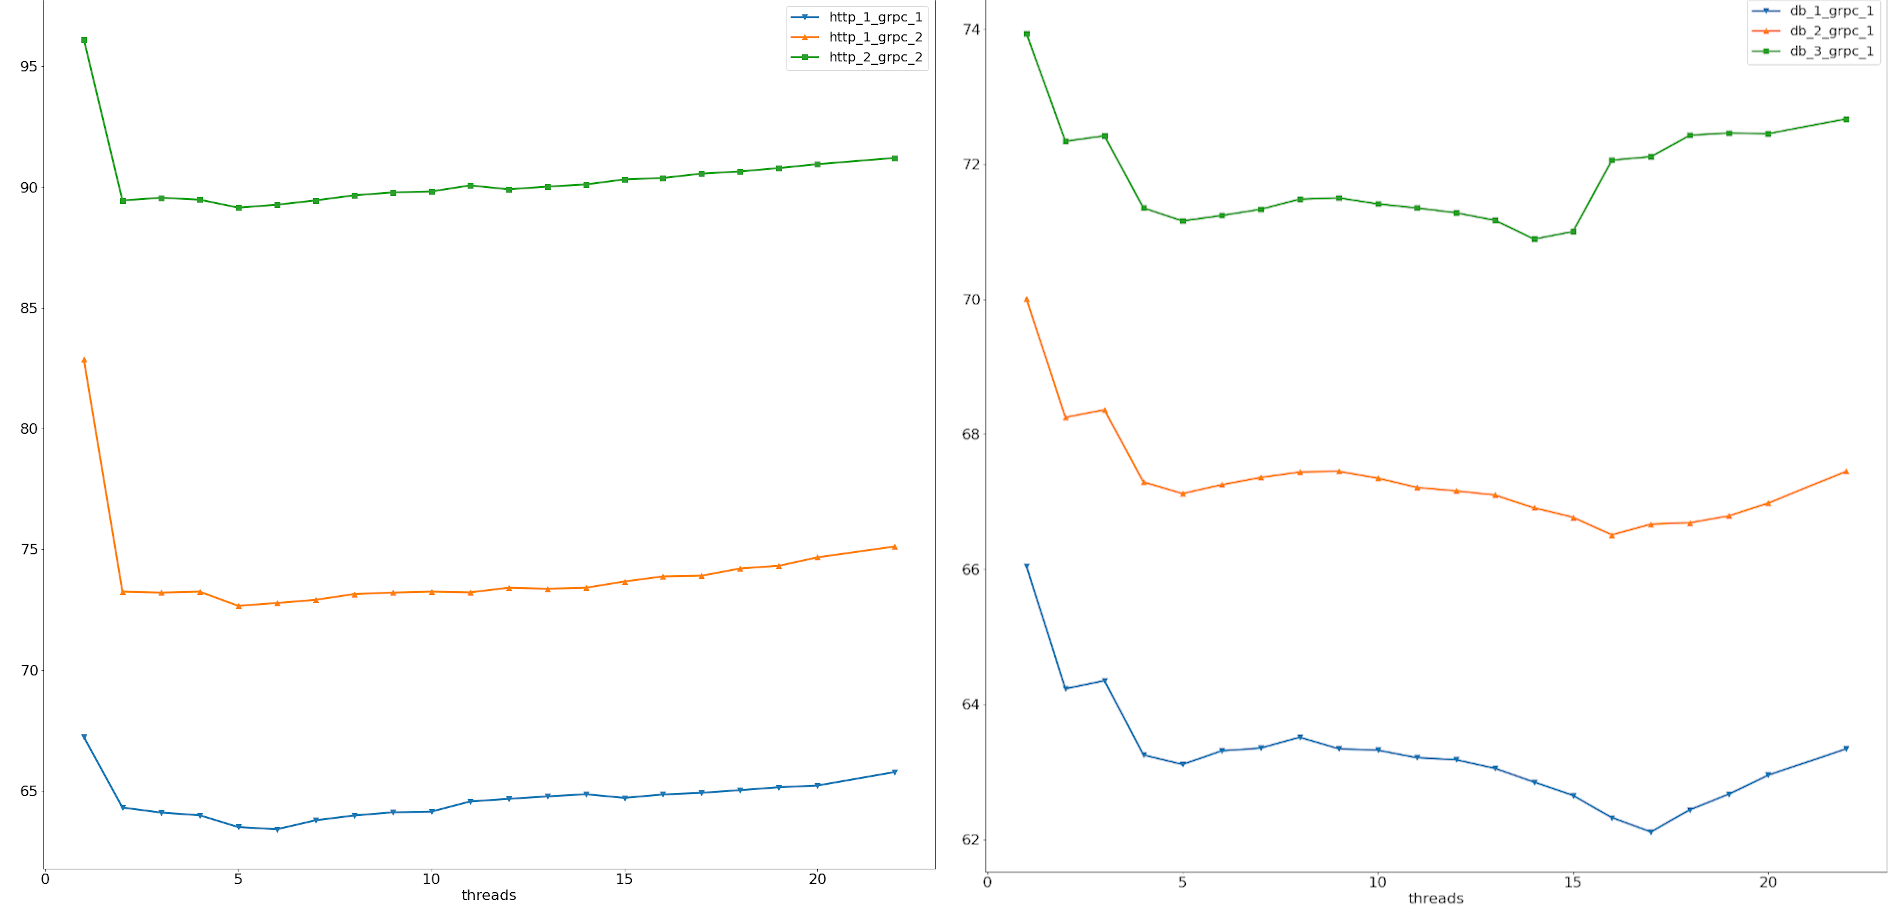
\includegraphics[scale=1]{figures/pool-http-db-db-grpc.png}
	\end{center}
	\caption{Left plot shows Thread pool size vs Average latency (millisecond) for number of database calls and grpc calls. \textbf{http\_1\_grpc\_2} represent that program has 1 http call and 2 grpc calls. Right plot shows Thread pool size vs Average latency (millisecond) for number of database calls and number of grpc calls.}
	\label{thread_pool_http_db_and_db_grpc}
\end{figure}

Based on previous experiment set, performance is evaluated for different thread pool sizes. Programs which contains different type of IO features are analyzed. In previous experiment sets for IO features,  there were only database call test. Programs with following IO features are evaluated,
\begin{itemize}
	\item gRPC calls
	\item Database calls
	\item Http calls
\end{itemize}

Implemented programs contains above IO features. This experiment is aimed to obtain to get thread pool size which gives the minimum latency. More details of the design is explained in chapter 3. Results are taken from  82 programs.

Figure \ref{thread_pool_database_and_http} and figure \ref{thread_pool_http_db_and_db_grpc} shows some results for thread pool size of 1 to 22. This range is selected because minimum of the average latency is always laid between this range. In order to verify the selected range, experiments are conducted for higher number of thread pool sizes. Those results showed only increase of average latency. 

From these experiments, thread pool size which gives minimum latency is obtained in order to feed the machine learning model. 

\section{Results comparison of machine learning models}

This section presents the results of machine learning models. The machine learning model can be expressed as follows,

$$ Optimal\:thread\:pool\:size = f(\:Program\:features)$$

After feature engineering steps, following features are selected to train the machine learning model.

\begin{itemize}
	\item Number of HTTP connector calls
	\item Number of Database connector calls
	\item Number of non-blocking gRPC connector calls
	\item Whether each type of connector calls lies inside a loop 
	\item Whether loops contain HTTP,Database or gRPCS calls (As separate features)
\end{itemize} 

Features are obtained by parsing the AST of Ballerina programs. Input of the training data set is above programming features and output is the optimal thread pool size which gives the minimum latency. Table \ref{tab:data_frame_with_results} shows the fragment of the data set.

\begin{figure}[htbp]
	\begin{center}
		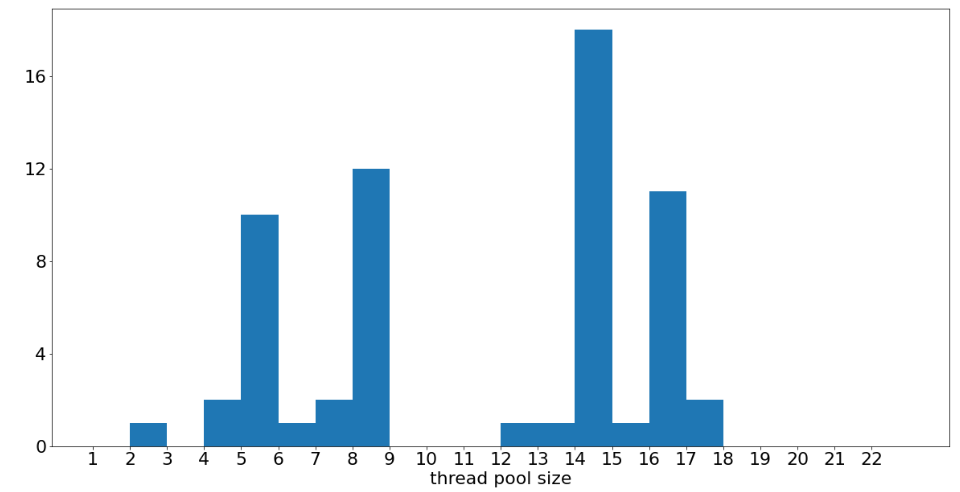
\includegraphics[scale=0.5]{figures/pool_size_dist.png}
	\end{center}
	\caption{No. of occurrences of optimal thread pool sizes.}
	\label{pool_size_dist}
\end{figure}

% Please add the following required packages to your document preamble:
% \usepackage{multirow}
\begin{table}[]
	\caption{Fragment of training data set}
	\label{tab:data_frame_with_results}
	\begin{tabular}{|l|l|l|l|l|l|l|}
		\hline
		\multirow{2}{*}{\textbf{Program}} & \multicolumn{5}{l|}{\textbf{Features}}                                                                                                                                                                                                                                                                                                                                                                    & \textbf{\begin{tabular}[c]{@{}l@{}}Optimal \\ thread \\ pool size\end{tabular}} \\ \cline{2-7} 
		& \textbf{\begin{tabular}[c]{@{}l@{}}No. of \\ database \\ calls\end{tabular}} & \textbf{\begin{tabular}[c]{@{}l@{}}No. of \\ HTTP \\ calls\end{tabular}} & \textbf{\begin{tabular}[c]{@{}l@{}}No. of\\ gRPC\\ calls\end{tabular}} & \textbf{\begin{tabular}[c]{@{}l@{}}No. loops \\ that contains\\ database \\ calls\end{tabular}} & \textbf{\begin{tabular}[c]{@{}l@{}}More \\ features...\end{tabular}} & \textbf{}                                                                       \\ \hline
		Program 1                         & 1                                                                            & 0                                                                        & 0                                                                      & 0                                                                                               & ...                                                                  & 14                                                                              \\ \hline
		Program 2                         & 1                                                                            & 2                                                                        & 0                                                                      & 0                                                                                               & ...                                                                  & 5                                                                               \\ \hline
		...                               & ...                                                                          & ...                                                                      & ...                                                                    & ...                                                                                             & ...                                                                  & ...                                                                             \\ \hline
	\end{tabular}
\end{table}

Then each following machine learning model is trained with the above data-set. In order to avoid over-fitting because of data set is small 5-fold cross validation is performed. For evaluation the performance of machine learning model 30\% of data is used as test data. Then following machine learning models are selected and evaluated the accuracy of each model.

This problem is originally a regression problem. But when it is analyzed the optimal thread pool size for each program, the distribution is very narrowed. Figure \ref{pool_size_dist} shows number of occurrences of each thread pool size. High frequency of optimal thread pool values can be seen around values of 5,8,14 and 16. Thus four classes can be created and reduce the machine learning model to classification problem as well. But there are some low frequency values around high frequency values also. For example around the value of 14, there are values of 12,13 and 15. Frequency of them is one. Those programs can be assigned to nearby class by observing the data set. Considering this fact results are shown for both classification and regression models. However, the accuracy of classification model is low compared to regression model. Results is presented in table \ref{tab:model-performance}.

\begin{itemize}
	
	\item XGBoost
	\item Support Vector Machine
	\item Decision Tree
	\item Random Forest
	
\end{itemize}

For regression models \acrfull{MAPE} and \acrfull{MSE} are evaluated. For classification models F1 score and accuracy are evaluated. When comparing models, it is clear that Decision Tree Regression model has the lowest \acrfull{MAPE} and \acrfull{MSE} values. The XGBoost Regression model is another good candidate. 

\begin{table}[]
	\caption{Evaluation of different machine learning model}
	\label{tab:model-performance}
	\begin{tabular}{|l|l|l|l|l|l|}
		\hline
		\multirow{2}{*}{\textbf{\begin{tabular}[c]{@{}l@{}}Machine \\ Learning\\ Model\end{tabular}}} & \multicolumn{3}{l|}{\textbf{Classification}}                                                                                                                 & \multicolumn{2}{l|}{\textbf{Regression}} \\ \cline{2-6} 
		& \textbf{Accuracy} & \textbf{\begin{tabular}[c]{@{}l@{}}F1 score\\ macro\end{tabular}} & \textbf{\begin{tabular}[c]{@{}l@{}}F1 score\\ weighted\end{tabular}} & \textbf{MAPE}        & \textbf{MSE}      \\ \hline
		XGBoost                                                                                       & 62.73\%           & 59.38\%                                                           & 62.29\%                                                              & 7.92\%               & 0.91              \\ \hline
		SVM                                                                                           & 59.09\%           & 45.08\%                                                           & 52.97\%                                                              & 30.06\%              & 13.41             \\ \hline
		\textbf{Decision Tree}                                                                        & 66.36\%           & 62.93\%                                                           & 67\%                                                                 & \textbf{6.79\%}      & \textbf{0.91}     \\ \hline
		Random Forest                                                                        		  & 68.59\%           & 61.58\%                                                           & 69\%                                                                 & 9.17\      & 1.55     \\ \hline
	\end{tabular}
\end{table}

\chapter{Conclusions}\label{chap:6}

\section{Introduction}

This chapter discusses the conclusion of the research project with regard to research questions defined in section \ref{sec:research_questions}. Furthermore, Limitations of the research and further implication of this research is discussed.

\section{Conclusions about research questions (aims/objectives)}

The initial objective of the research was finding a server architecture that would result in the best performance for a given Ballerina program. Initially, three server architectures were implemented in Ballerina run-time by removing,adding and modifying existing components. Server architectures were chosen based on previous studies \cite{comparing_high_performance_multi_core,comp_ac,flash_server,seda}. Number of thread pools (i.e stages in SEDA) and configuration of thread pools were major points when differentiating the server architectures. Performance of Current Ballerina architecture,Netty OIO and Removed Ballerina scheduler (specifically scheduler thread pool ) were evaluated against different types of programs. Additionally, two variations of original Ballerina architecture were implemented by changing the size of the scheduler thread pool. Programs consisted of either CPU intensive or IO intensive features. Metrics such as throughput, average latency, standard deviation are evaluated. Experiments in the first phase showed that removing the scheduler thread pool resulted in higher throughput and lower latency for all programs. Furthermore, Netty OIO gave  the worst performance for every program. Therefore, we could not identify an architecture that would result in the best performance  for a given program among selected architectures. 


Since changing thread pool size affected differently for IO and CPU intensive programs, we tried to answer the second research question which is optimizing performance of server architecture by tuning the thread pool size. There are several studies \cite{xu2004performance,thread_pool_analysis,math_aproach_thread_pool_tuning,syer2011identifying,linfeng2017design} which try to provide analytical models for thread pool optimization. However, none of them have addressed the thread pool optimization based on different program characteristics. Scheduler thread pool in current ballerina architecture is selected over removed scheduler architecture in order to tune because of stability issues referred in section when load to the web server (no. of concurrent users) is increased. New programs were added for testing which have different IO characteristics (Database calls, HTTP calls, gRPC calls). Experiments were designed to measure impact of thread pool size for different IO features in programs. We were able to determine the impact of thread pool size for different programs which consisted of different IO features. We were able to find thread pool size which gives minimum average latency for each program.


The final objective was deriving a model to predict optimal thread pool size based on a given set of programming features. A machine learning model was trained in order to answer the last research question. The model takes input as features in the given ballerina program (i.e Number of database calls, HTTP calls, gRPC calls, loops) and estimates optimal thread pool size as output. Among several machine learning models, the Decision Tree regression model was chosen based on evaluation metrics. Hence, we were able to devise a model that estimates the thread pool size for a given Ballerina program.

\section{Conclusions about research problem}

In this research, we are able to propose a model to estimate optimal thread pool size for a given Ballerina program. Ballerina's native representation of remote IO calls a.k.a connector calls and other web service oriented features supported to extract these features directly from source code by parsing AST tree. The combination of all modules makes it easier to decide the optimal thread pool size for Ballerina scheduler prior to execution of the program. This process can be integrated into the compilation process of the Ballerina program resulting in automatic thread pool size configuration in compiled code. The result of this study can be used as proof of concept for performance estimation based on programming features.

Furthermore, heuristic rules such as deciding the number of thread pool size as twice the number of CPU \cite{thread_pool_analysis} is not resulting in optimal performance has been proven when analyzing the results of the first phase. In figures \ref{phase-1-database-all-architectures},\ref{phase-1-prime-small-all-architectures},\ref{phase-1-prime-medium-all-architectures},\ref{phase-1-prime-large-all-architectures},\ref{phase-1-file-read-all-architectures} , (Note that \textit{scheduler x2} represent 4 times the number of CPUs and \textit{scheduler x4} results 8 times the number of CPUs ) we can see that performance is better when the number of threads are 4 times the number of CPUs than the current ballerina architecture where default thread pool size is 2 times the number of CPUs for all tested program types. 


\section{Limitations}

There are a number of limitations that occurred while progressing the research. In the first phase of the research we analyzed both CPU intensive and IO intensive applications. However, when building the machine learning model it was difficult to extract CPU intensive features directly from the source code.Thus, only IO characteristics were considered which were able to parse from source code. As an example, we can model the CPU intensive behaviors as number of variable assignment, comparisons and arithmetic operations then it is possible to extract this information from source code. But when 3rd party library functions calls are happening, it is not able to derive this information directly from the source code. This requires, analysis of compiled byte code than source code. Thus, this study did not explore that level.

Furthermore, results of the experiment can be subject to the environment of the machine where the server is deployed. The effect of the amount of RAM number of the CPU is not analyzed in this research.

Also, performance results can be subject to run time variables as well. This study only provides static analysis. As an example, the number of times that particular loop is executing can be depended on a variable. Some paths of the program may never get executed. Thus, for a given program features that are affected at run time may differ from the static information.



\section{Implications for further research}

For future studies this proof of concept can be made as the ground with combination of above limitations. We are able to prove that performance of web servers can be modeled based on program features. In this research we only considered the Ballerina language. Same set of experiments can be conducted for other frameworks and languages. If we can extract information from compiled code (byte-code in java) we can integrate total number of expressions, assignment, comparisons, loops and if clauses including 3rd party libraries as well. Then we can build an accurate model which includes both IO and CPU intensive features. Moreover, we can get relation among Number of CPU, Amount of RAM etc by running this model in multiple environments.     


\newpage
\renewcommand{\bibname}{References}

\newcommand{\theHalgorithm}{\arabic{algorithm}}

\newcommand{\alglinelabel}{%
	\addtocounter{ALC@line}{-1}% Reduce line counter by 1
	\refstepcounter{ALC@line}% Increment line counter with reference capability
	\label% Regular \label
}


\appendix
\chapter{Publications}
\chapter{Diagrams}
\chapter{Code Listings} \label{appendix:c}

Test programs and AST parser implementation can be found at \url{https://github.com/lakinduakash/ballerina-microbenchmarks} \cite{benchmark_implementation}. Web sever architecture implementation can be found at \url{https://github.com/lakinduakash/ballerina-lang} \cite{ballerina_architectures}
 
\lstinputlisting[language=Java, caption=Netty OIO Implementaion]{codes/DefaultHttpWsConnectorFactory.java}

\lstinputlisting[language=Bash, caption=Building Ballerina environment]{codes/ballerina-build-only.sh}

\lstinputlisting[language=Bash, caption=Running Ballerina tests ]{codes/ballerina-run-only.sh}

\lstinputlisting[language=Bash, caption=Running Ballerina with different thread pool sizes]{codes/run-all.sh}

\lstinputlisting[language=Bash, caption=Running Jmeter]{codes/jmeter-run-only.sh}

\lstinputlisting[language=Bash, caption=Running Ballerina tests]{codes/bal.Dockerfile}

\lstinputlisting[language=Html, caption=Jmeter Test plan]{codes/Test_Plan_General_4_params.jmx}

%\lstinputlisting[language=Java, caption=Ballerina test cases - Not included full set]{codes/main.bal}
\bibliography{ms}
\end{document}